\chapter{Object recognition}


\begin{description}
    \item[Vision] \marginnote{Vision}
        Process that, from images of the external world, 
        produces a description without irrelevant information (i.e. interference) useful to the viewer.

        This description includes information such as what is in the world and where it is.

        \begin{remark}
            Vision is the most important sense in primates (i.e. in case of conflicts between senses, vision is usually prioritized).
        \end{remark}

        \begin{remark}
            Vision is also involved in memory and thinking.
        \end{remark}

        \begin{remark}
            The two main tasks for vision are:
            \begin{itemize}
                \item Object recognition.
                \item Guiding movement.
            \end{itemize}
            These two functions are mediated by (at least) two pathways that interact with each other.
        \end{remark}


    \item[Vision Bayesian modeling] \marginnote{Bayesian modeling}
        Vision can be modeled using Bayesian theory.
        
        Given an image $I$ and a stimulus $S$, an ideal observer uses some prior knowledge (expectation) of the stimulus ($\mathcal{P}(S)$)
        and input sensory data ($\prob{I | S}$) to infer the most probable interpretation of the stimulus in the image:
        \[ \mathcal{P}(S | I) = \frac{\mathcal{P}(I | S) \mathcal{P}(S)}{\mathcal{P}(I)} \]

        \begin{remark}
            Prior knowledge is learned from experience. 
            It could be related to the shape of the object, the direction of the light or the fact that objects cannot overlap.
        \end{remark}

        \begin{remark}
            If the image is highly ambiguous, prior knowledge contributes more to disambiguate it.
        \end{remark}

        \begin{figure}[H]
            \centering
            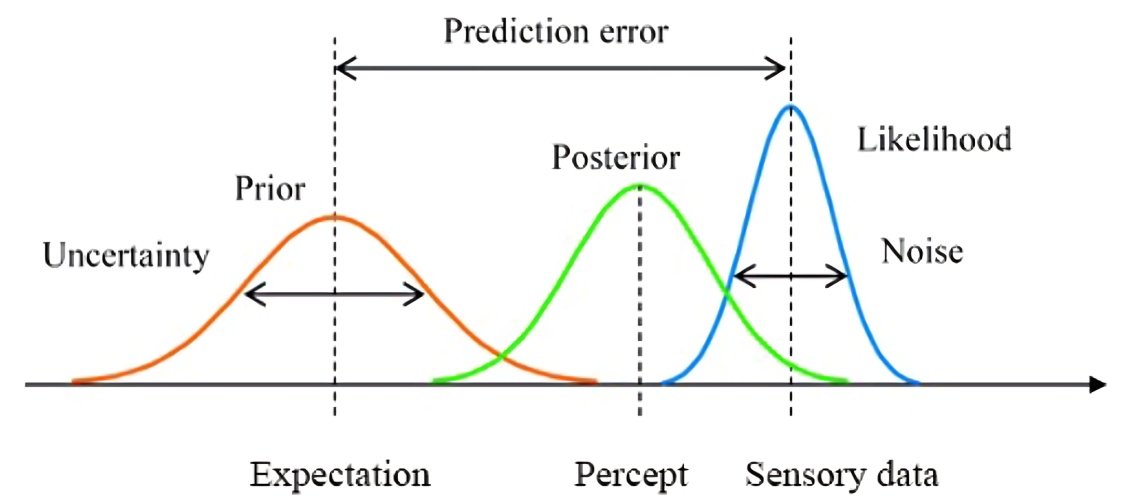
\includegraphics[width=0.4\linewidth]{./img/vision_bayesian.png}
        \end{figure}

        \begin{description}
            \item[Feed-forward processing] Involves the likelihood $\prob{I | S}$.
            \item[Feed-back processing] Involves the prior $\mathcal{P}(S)$.
        \end{description}

        \begin{remark}
            Perception integrates both feed-forward and feed-back processing.
        \end{remark}


    \item[Vision levels] \marginnote{Vision levels}
        A visual scene is analyzed at three levels:
        \begin{descriptionlist}
            \item[Low level]
                Processes simple visual attributes captured by the retina such as local contrast, orientation, color, depth and motion.

            \item[Intermediate level] 
                Low-level features are used to parse the visual scene (i.e. local features are integrated into the global image).
                This level is responsible for identifying boundaries and surfaces belonging to the same object and 
                discriminating between foreground and background objects.
                % \begin{example}
                %     Local orientation is integrated into global contours, local features are assembled into surfaces, 
                %     the shapes of surfaces are identified, \dots
                % \end{example}

            \item[High level] 
                Responsible for object recognition.
                
                Once the objects have been recognized, they can be associated with memories of shapes and meaning.

                \begin{casestudy}[Agnosia]
                    Patients with agnosia have their last level of vision damaged.
                    They can see (e.g. avoid obstacles) but cannot recognize object or get easily confused.
                \end{casestudy}
        \end{descriptionlist}

        \begin{figure}[H]
            \centering
            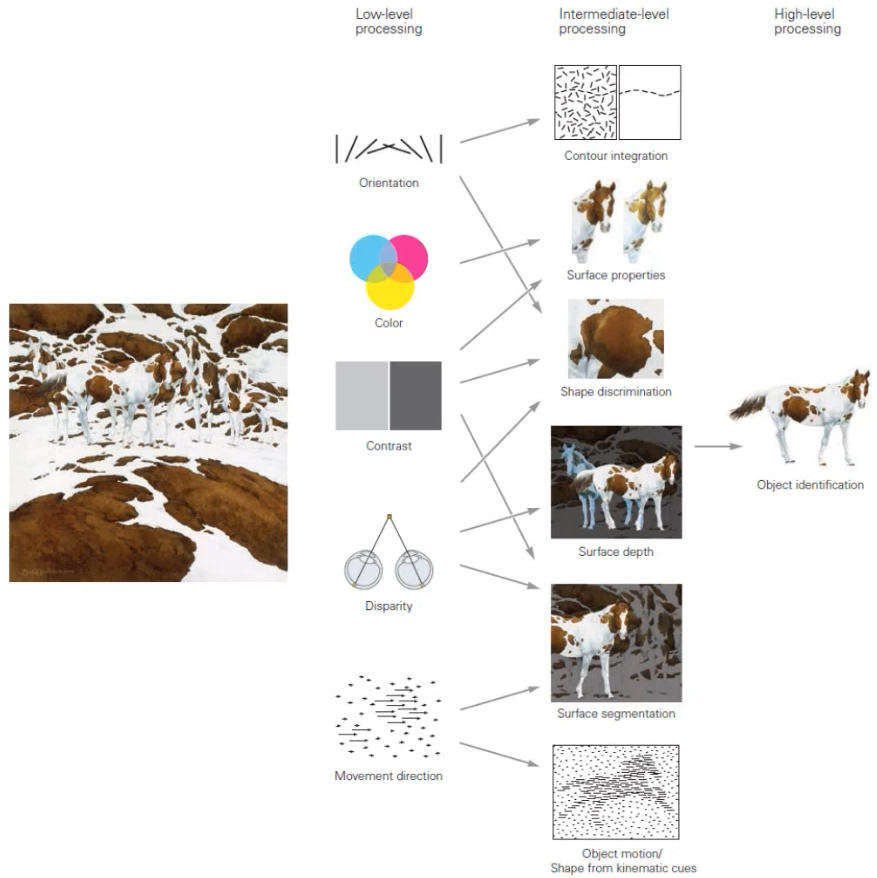
\includegraphics[width=0.55\linewidth]{./img/vision_levels.png}
        \end{figure}
\end{description}



\section{Pathways}

\begin{description}
    \item[Retino-geniculo-striate pathway] \marginnote{Retino-geniculo-striate pathway}
        Responsible for visual processing.
        It includes the:
        \begin{itemize}
            \item Retina.
            \item Lateral geniculate nucleus (LGN) of the thalamus.
            \item Primary visual cortex (V1) or striate cortex.
            \item Extrastriate visual areas (i.e. beyond the area V1).
        \end{itemize}

        \begin{figure}[H]
            \centering
            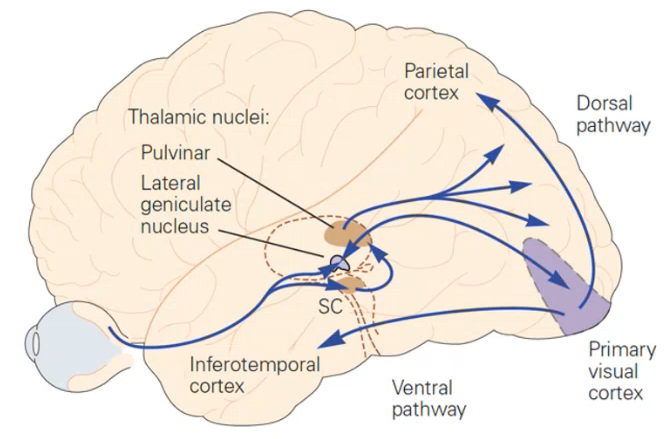
\includegraphics[width=0.35\linewidth]{./img/vision_pathway.png}
        \end{figure}

        
    \item[Ventral pathway] \marginnote{Ventral pathway}
        Responsible for object recognition.
        It extends from the area V1 to the temporal lobe (feed-forward processing).

        \begin{remark}
            This pathway emphasizes color.
        \end{remark}

        \begin{remark}
            The connection from the frontal lobe encodes prior knowledge (feed-back processing).
        \end{remark}

    \item[Dorsal pathway] \marginnote{Dorsal pathway}
        Responsible for movement guiding.
        It connects the V1 area with the parietal lobe and then with the frontal lobe.

        \begin{remark}
            This pathway is colorblind.
        \end{remark}
\end{description}

\begin{remark}
    The ventral and dorsal pathways are highly connected and share information.
\end{remark}

\begin{remark}
    All connections in the ventral and dorsal pathways are reciprocal (i.e. bidirectional).
\end{remark}

\begin{figure}[H]
    \centering
    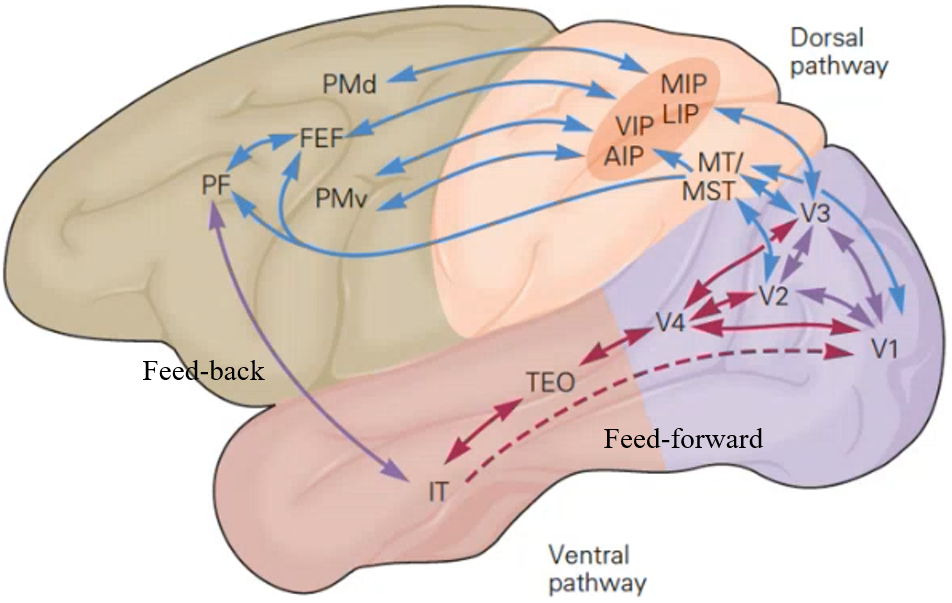
\includegraphics[width=0.4\linewidth]{./img/ventral_dorsal_pathways.png}
\end{figure}


\section{Neuron receptive field}
\begin{description}
    \item[Single-cell recording] \marginnote{Single-cell recording}
        Technique to record the firing rate of neurons.
        A fine-tipped electrode is inserted into the animal's brain to record the action potential of a single neuron.
        
        This method is highly invasive but allows to obtain high spatial and temporal readings of the neuron firing rate while distinguishing excitation and inhibition.

        \begin{remark}
            On a theoretical level, neurons can fire a maximum of $1000$ times per second.
            This may actually happen in exceptional cases.
        \end{remark}

    
    \item[Receptive field] \marginnote{Receptive field}
        Region of the visual scene at which a particular neuron will respond if a stimulus falls within it. 

        \begin{remark}
            The receptive field of a neuron can be described through a Gaussian.
        \end{remark}

        \begin{casestudy}
            A monkey is trained to maintain fixation at a point on a screen.
            Then, stimuli are presented in various positions of the visual field.

            It has been seen that a particular neuron fires vigorously only when a stimulus is presented in a particular area of the screen.

            The response is the strongest at the center of the receptive field and gradually declines when the stimulus moves away from the center.

            \begin{figure}[H]
                \centering
                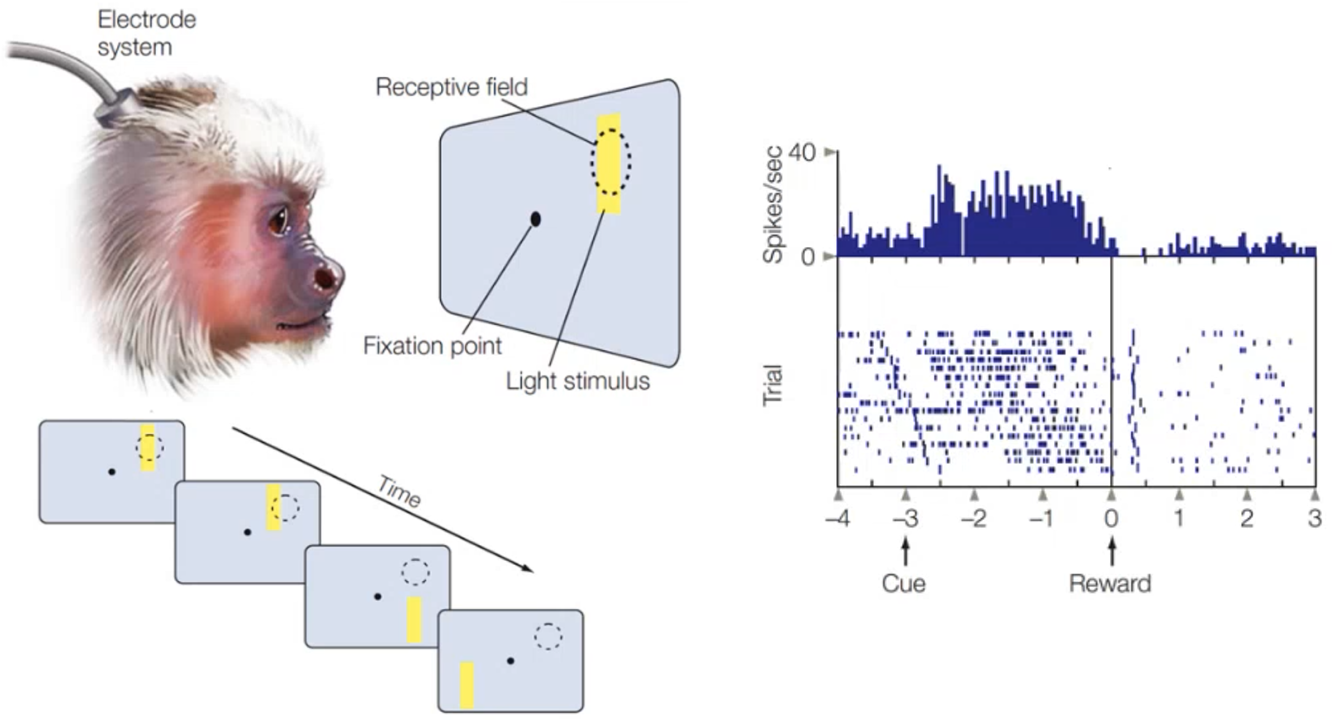
\includegraphics[width=0.55\linewidth]{./img/receptive_field_monkey.png}
            \end{figure}
        \end{casestudy}

        \begin{remark}
            Neurons might only react to a specific type of stimuli in the receptive field (e.g. color, direction, \dots).

            \begin{casestudy}
                It has been seen that a neuron fires only if a stimulus is presented in its receptive field while moving upwards.
            \end{casestudy}
        \end{remark}

    
    \item[Retinotopy] \marginnote{Retinotopy}
        Mapping of visual inputs from the retina (i.e. receptive field) to the neurons.

        There is a non-random relationship between the position of the neurons in the visual areas (V1, V2, V4):
        their receptive fields form a 2D map of the visual field in such a way that 
        neighboring regions in the visual image are represented by adjacent regions of the visual cortical area
        (i.e. the receptive fields are spatially ordered).

        \begin{figure}[H]
            \centering
            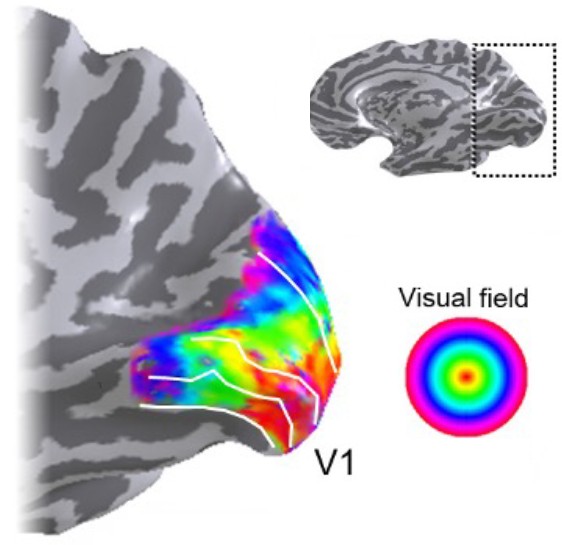
\includegraphics[width=0.3\linewidth]{./img/retinotopy.png}
            \caption{\parbox[t]{0.45\linewidth}{Mapping from the visual field to the neurons in the primary visual cortex (V1)}}
        \end{figure}

        \begin{description}
            \item[Eccentricity] \marginnote{Eccentricity}
                The diameter of the receptive field is proportional to the wideness of the visual angle.

                \begin{figure}[H]
                    \centering
                    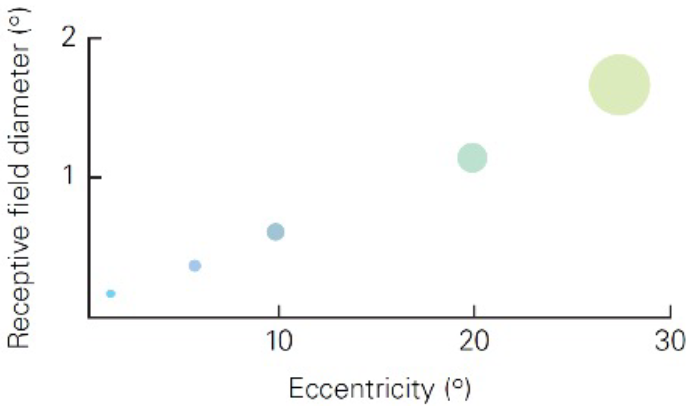
\includegraphics[width=0.35\linewidth]{./img/eccentricity.png}
                    \caption{\parbox[t]{0.45\linewidth}{Relationship between visual angle and receptive field diameter}}
                \end{figure}

            \item[Cortical magnification] \marginnote{Cortical magnification}
                The neurons (retinal ganglion cells, RGCs) responsible for the center of the visual field (fovea)
                have a visual angle of about $0.1^\circ$ while the neurons at the visual periphery reach up to $1^\circ$ of visual angle.

                Accordingly, more cortical space is dedicated to the central part of the visual field.
                This densely packed amount of smaller receptive fields allows for the highest spatial resolution at the center of the visual field.

                \begin{figure}[H]
                    \centering
                    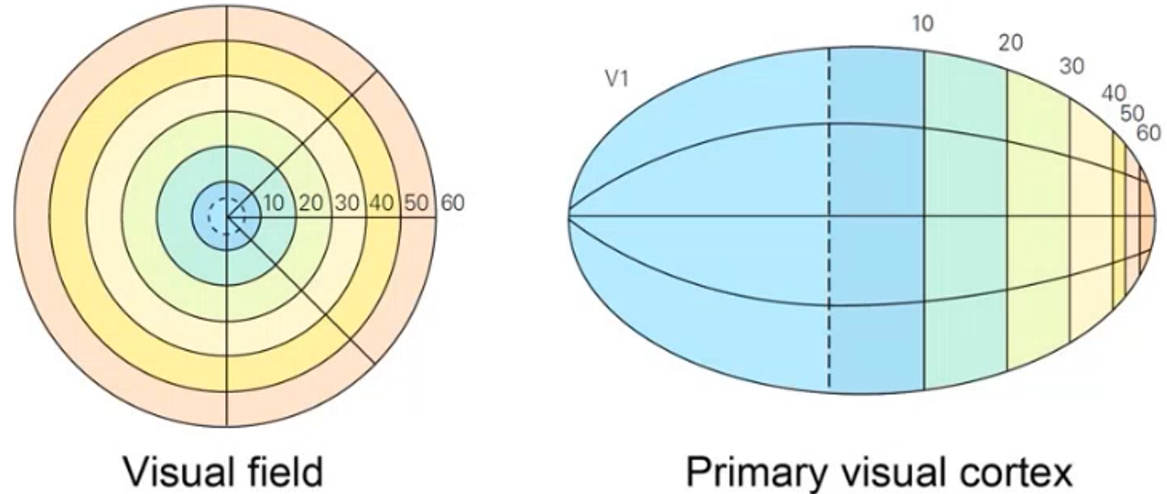
\includegraphics[width=0.4\linewidth]{./img/cortical_magnification.png}
                    \caption{Cortical magnification in V1}
                \end{figure}

                \begin{remark}
                    The brain creates the illusion that the center and the periphery of vision are equal.
                    In reality, the periphery has less resolution and is colorblind.
                \end{remark}
        \end{description}

    \item[Hierarchical model of receptive field]
        The processing of some information in the visual image is done through an incremental convergence of information
        in a hierarchy of receptive fields of neurons.
        Along the hierarchy the size of the receptive field increases.
\end{description}


\section{Retina cells}

\begin{description}
    \item[Photoreceptor] \marginnote{Photoreceptor}
        Specialized neurons that are hyperpolarized in bright regions and depolarized in dark regions.
        \begin{figure}[H]
            \centering
            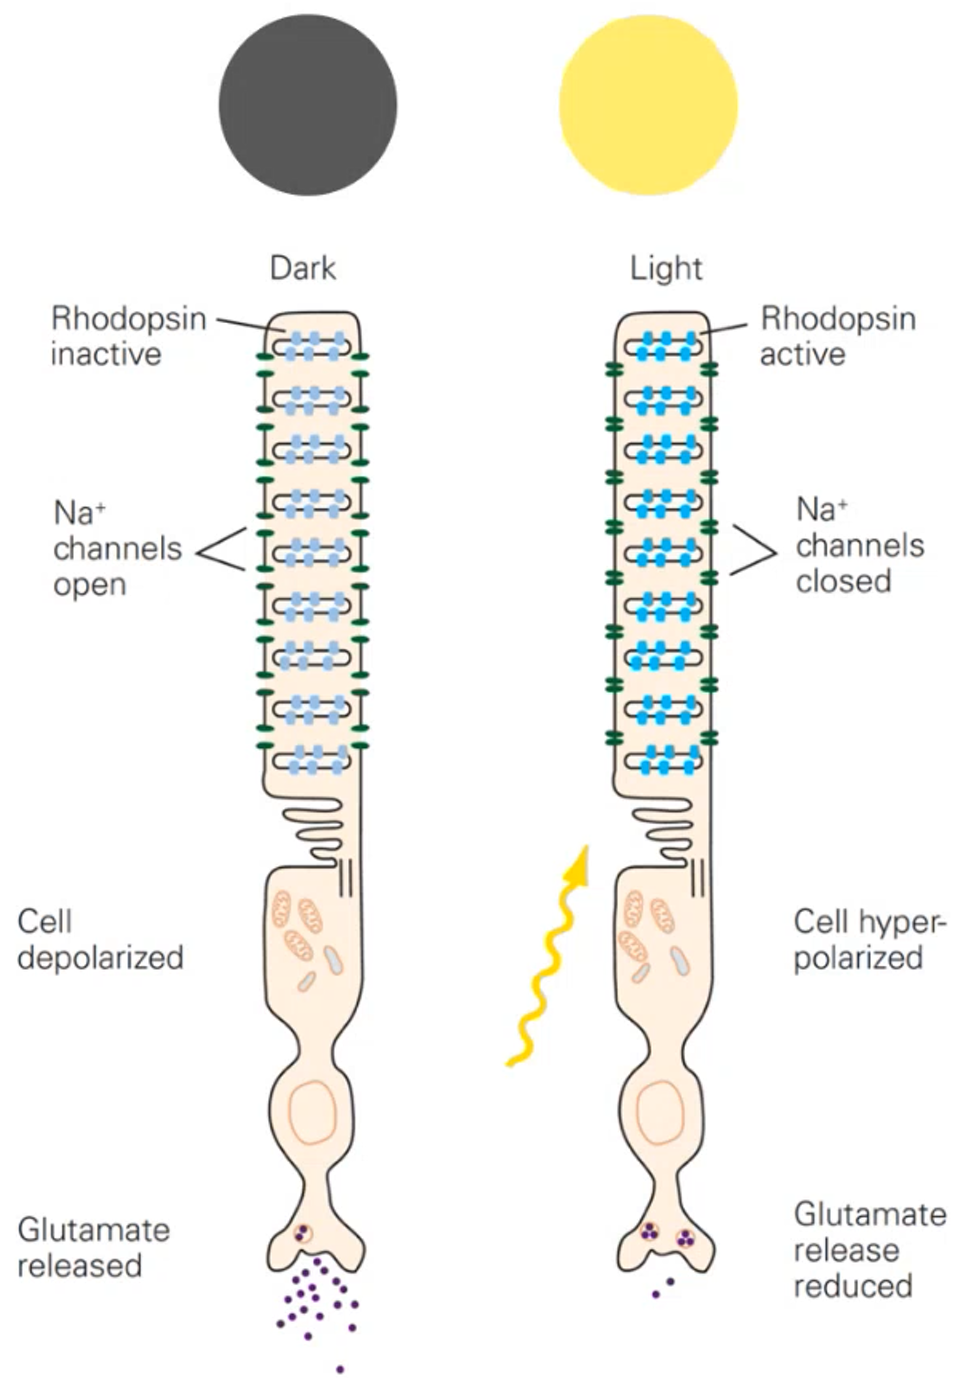
\includegraphics[width=0.3\linewidth]{./img/photoreceptor.png}
        \end{figure}

        \begin{remark}
            They are the first layer of neurons in the retina.
        \end{remark}


    \item[Retinal ganglion cell (RGC)] \marginnote{Retinal ganglion cell (RGC)}
        Neurons of the visual cortex with a circular receptive field.
        They are categorized into:
        \begin{descriptionlist}
            \item[ON-center] \marginnote{ON-center cells}
                RGCs that are activated in response to a bright stimulus in the center of the receptive field.
            \item[OFF-center] \marginnote{OFF-center cells}
                RGCs that are activated in response to a dark stimulus in the center of the receptive field.
        \end{descriptionlist}

        \begin{remark}
            They are the last layer of neurons in the retina, before entering LGN of the thalamus.
        \end{remark}

        The receptive field of RGCs is composed of two concentric areas. 
        The inner one acts according to the type of the cell (ON-center/OFF-center)
        while the outer circle acts antagonistically to the inner area.

        \begin{remark}
            A uniform stimulus that covers the entire receptive field of an RGC produces a weak or no response.
        \end{remark}

        \begin{remark}
            RGCs are not responsible for distinguishing orientation or lines.
        \end{remark}

        \begin{figure}[H]
            \centering
            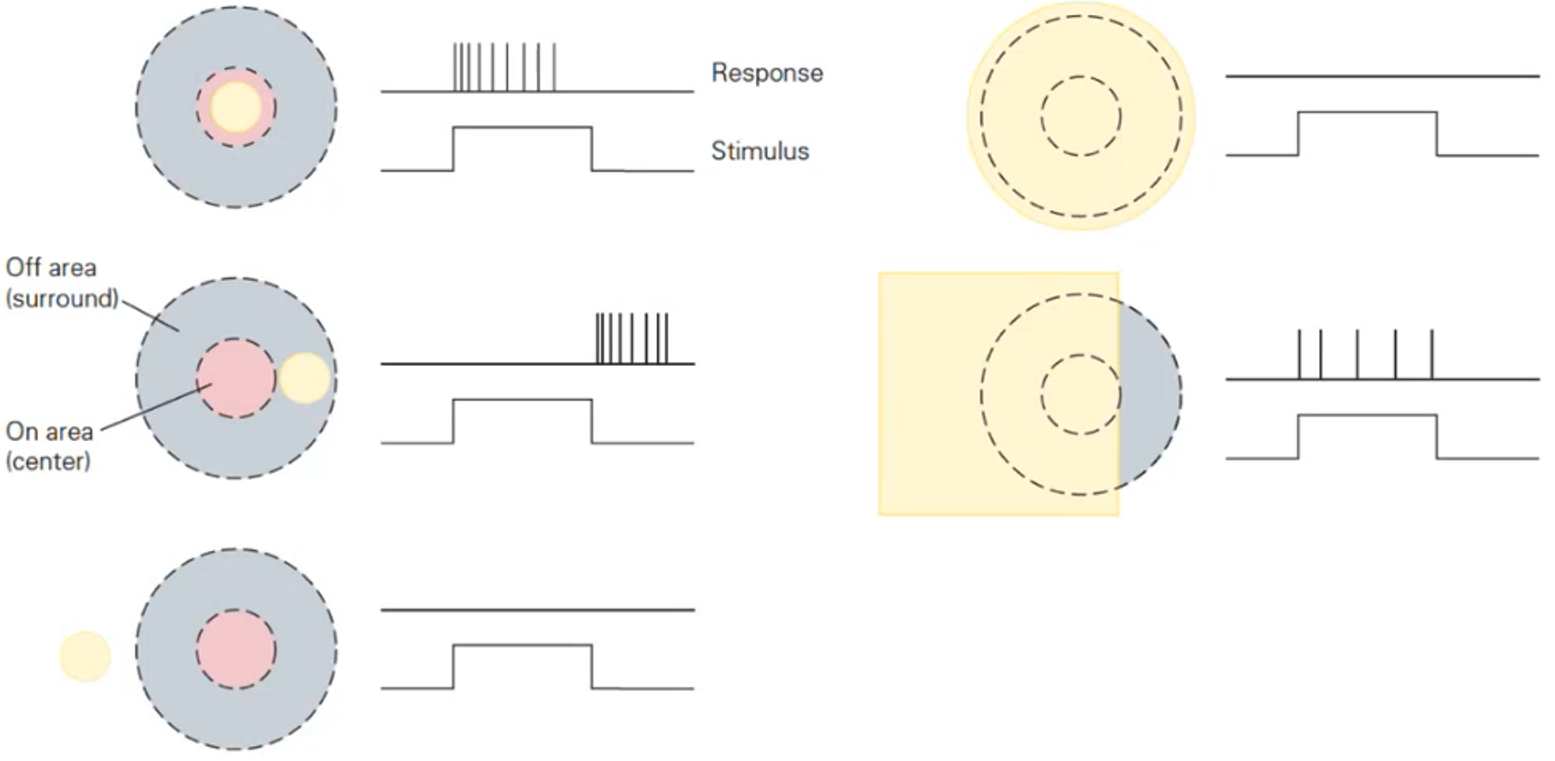
\includegraphics[width=0.6\linewidth]{./img/on_off_center.png}
            \caption{Responses of an ON-center RGC}
        \end{figure}

        \begin{remark}
            The response of RGCs can be described by two Gaussians: 
            one is positive with a narrow peak and represents the response at the center 
            while the other is negative with a wide base and covers both the inner and outer circles.
            Their difference represents the response of the cell (receptive field profile).

            \begin{figure}[H]
                \centering
                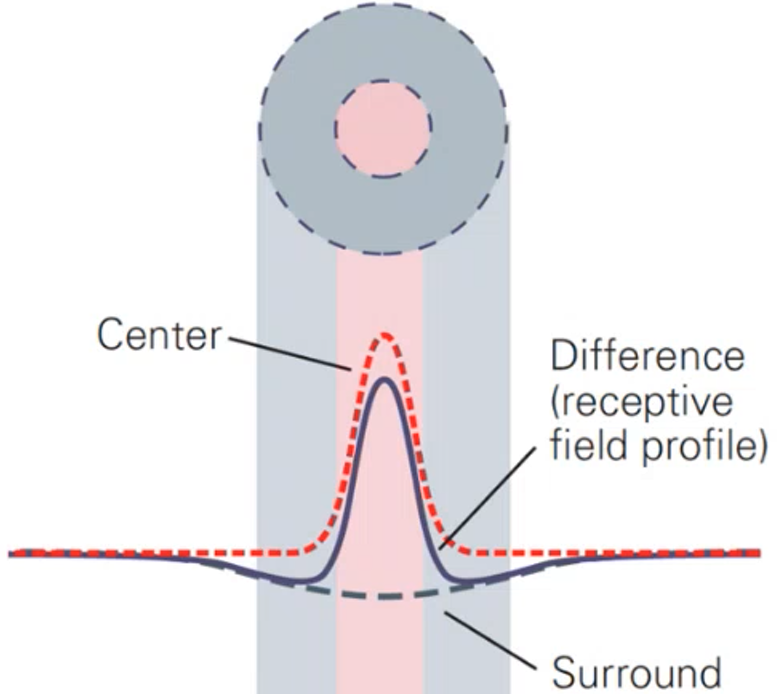
\includegraphics[width=0.2\linewidth]{./img/visual_gaussian.png}
            \end{figure}
        \end{remark}

        \begin{description}
            \item[Band-pass behavior] \marginnote{Band-pass behavior}
                The visual system of humans has a band-pass behavior: it only responds to a narrow band of intermediate frequencies
                and is unable to respond to spatial frequencies that are too high or too low 
                (as they get canceled by the two antagonistic circles).

                \begin{figure}[H]
                    \centering
                    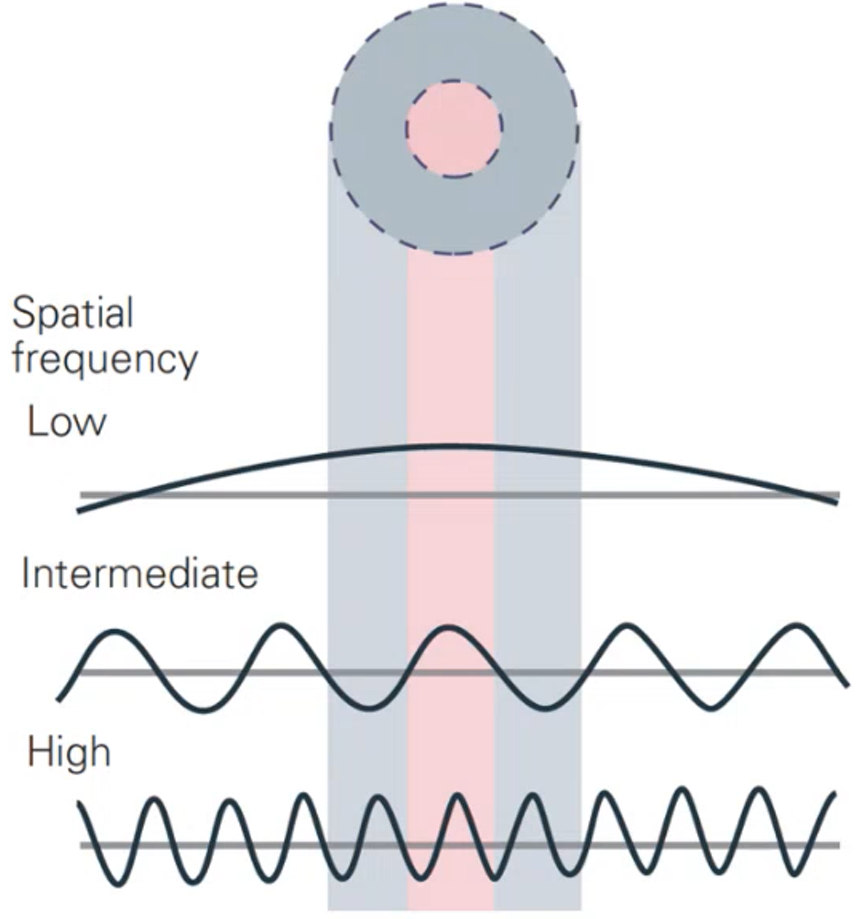
\includegraphics[width=0.2\linewidth]{./img/visual_frequencies.png}
                \end{figure}
        \end{description}
\end{description}



\section{Area V1 cells}


\subsection{Simple cells}
\marginnote{Simple cells}

Neurons that respond to a narrow range of orientations and spatial frequencies.

This is the result of the alignment of different circular receptive fields of the LGN cells (which in turn receive their input from RGCs).

\begin{figure}[H]
    \centering
    \begin{subfigure}{0.45\linewidth}
        \centering
        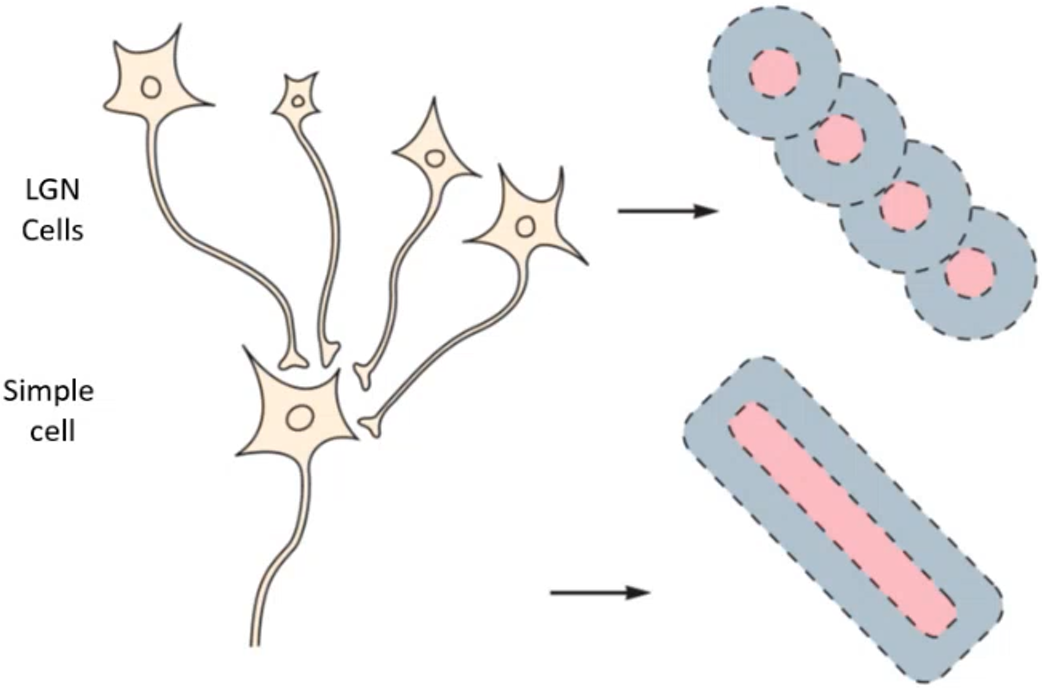
\includegraphics[width=0.9\linewidth]{./img/v1_simple_cell.png}
    \end{subfigure}
    \begin{subfigure}{0.45\linewidth}
        \centering
        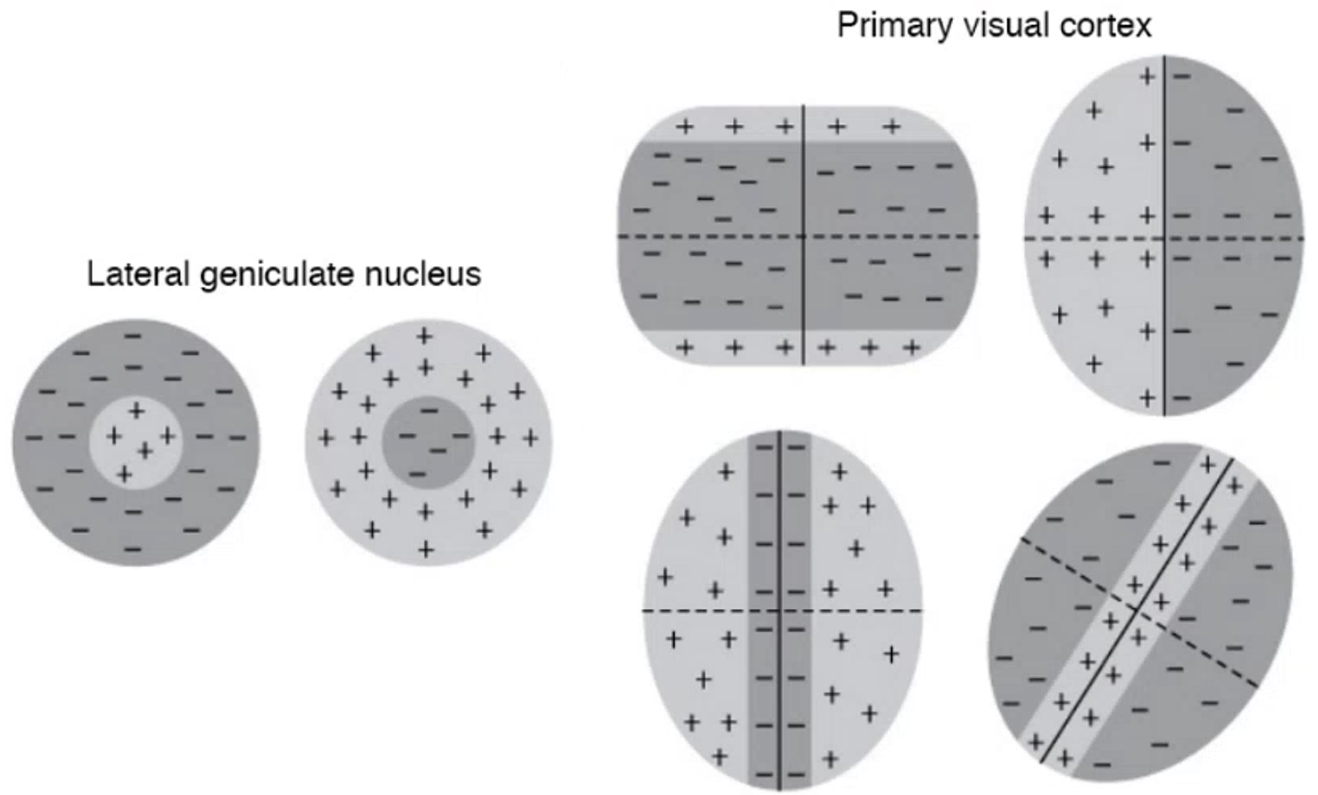
\includegraphics[width=0.9\linewidth]{./img/v1_simple_cells_visual.png}
    \end{subfigure}
\end{figure}

\begin{casestudy}
    In monkeys, the neurons of the LGN have non-oriented circular receptive fields.
    Still, simple cells are able to perceive specific orientations.
\end{casestudy}

\begin{description}
    \item[Simple cells model] 
        The stages of computation in simple cells are:
        \begin{enumerate}
            \item Linear filtering through a weighted sum of the image intensities done by the receptive field (i.e. convolutions).
            \item Rectification (i.e. thresholding with non-linearity) to determine if the neuron has to fire.
        \end{enumerate}

        \begin{figure}[H]
            \centering
            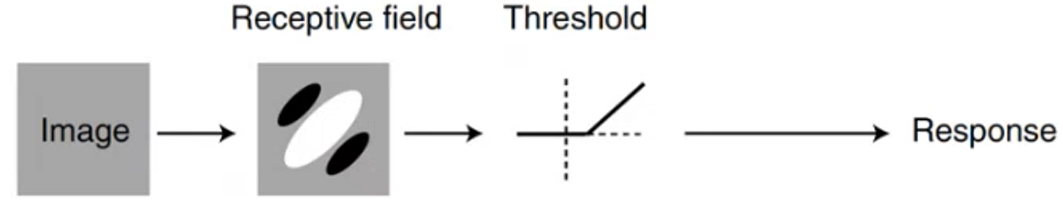
\includegraphics[width=0.4\linewidth]{./img/simple_cell_model.png}
        \end{figure}
\end{description}


\subsection{Complex cells}
\marginnote{Complex cells}

Neurons with a rectangular receptive field larger than simple cells.
They respond to linear stimuli with a specific orientation and move in a particular direction (position invariance).

\begin{remark}
    At this stage, the position of the stimulus is not relevant anymore as the ON and OFF zones of the previous cells are mixed.
\end{remark}

\begin{figure}[H]
    \centering
    \begin{subfigure}{0.45\linewidth}
        \centering
        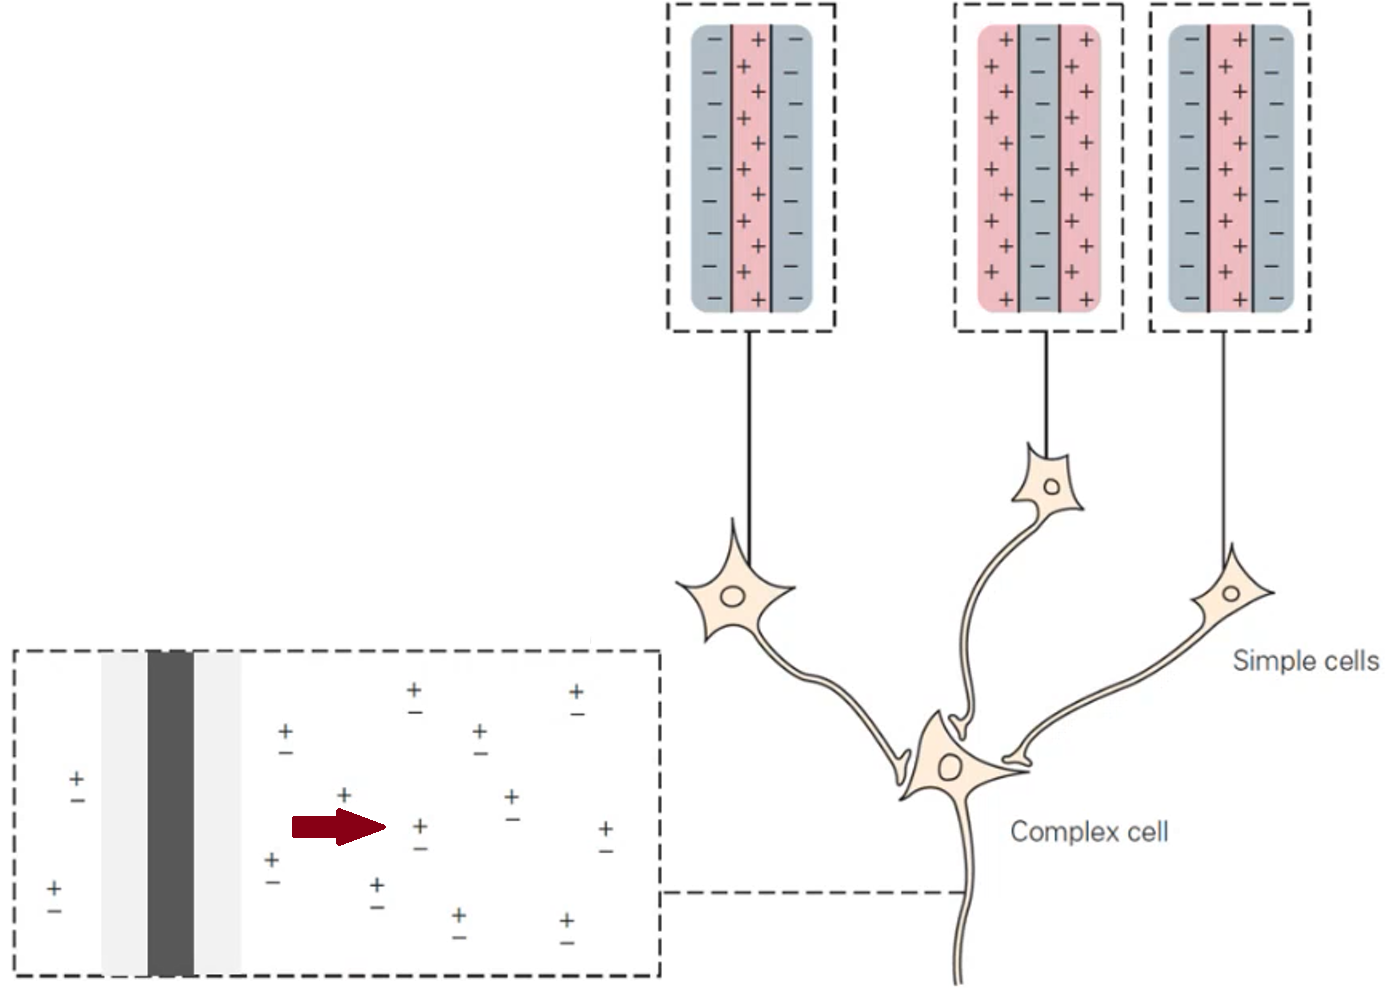
\includegraphics[width=0.9\linewidth]{./img/complex_cell.png}
    \end{subfigure}
    \begin{subfigure}{0.45\linewidth}
        \centering
        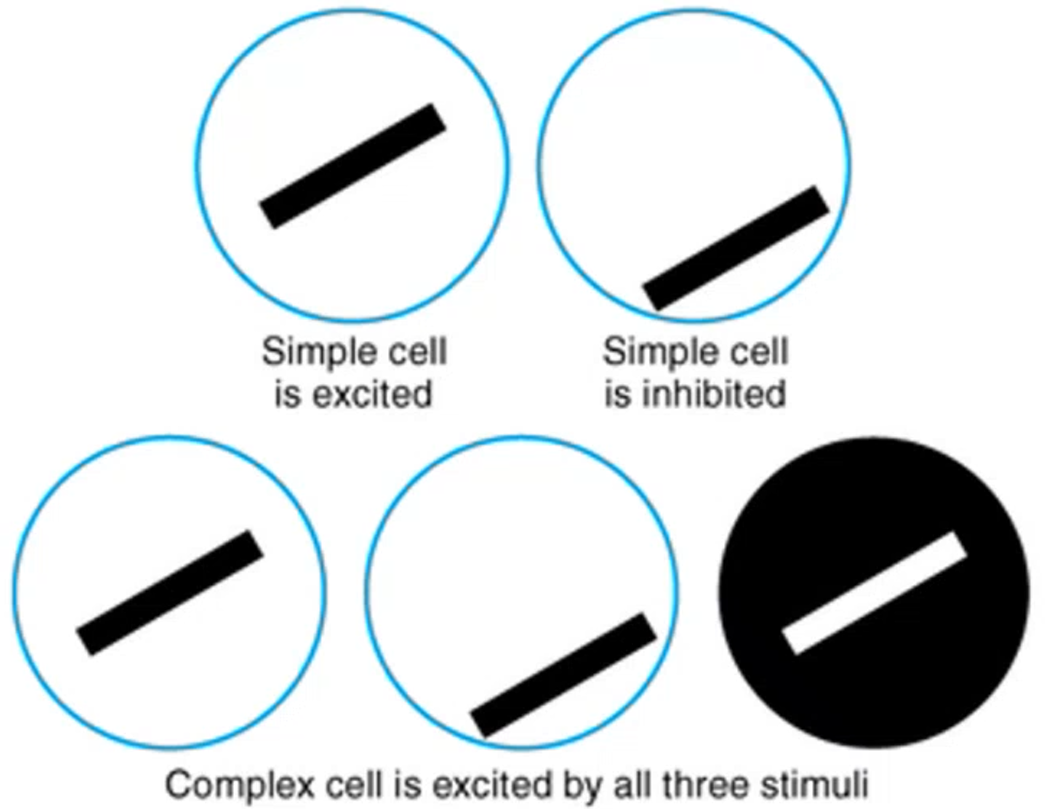
\includegraphics[width=0.6\linewidth]{./img/complex_cell_stimuli.png}
    \end{subfigure}
\end{figure}

\begin{description}
    \item[Complex cell model]
        The stages of computation in complex cells are:
        \begin{enumerate}
            \item Linear filtering of multiple receptive fields.
            \item Rectification for each receptive field.
            \item Summation of the response.
        \end{enumerate}

        \begin{figure}[H]
            \centering
            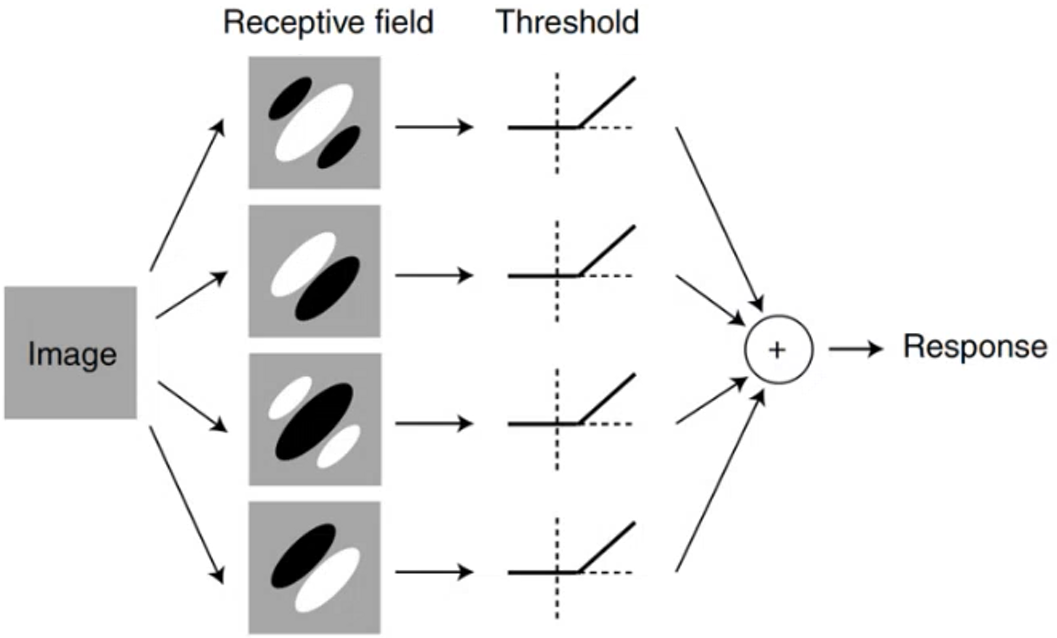
\includegraphics[width=0.4\linewidth]{./img/complex_cell_model.png}
        \end{figure}
\end{description}


\subsection{End-stopped (hypercomplex) cells}
\marginnote{End-stopped cells}

Neurons whose receptive field has an excitatory region surrounded by one or more inhibitory regions all with the same preferred orientation.

This type of cell responds to short segments, long curved lines (as the tail of the curve that ends up in the inhibition region is not the preferred orientation)
or to angles.

\begin{figure}[H]
    \centering
    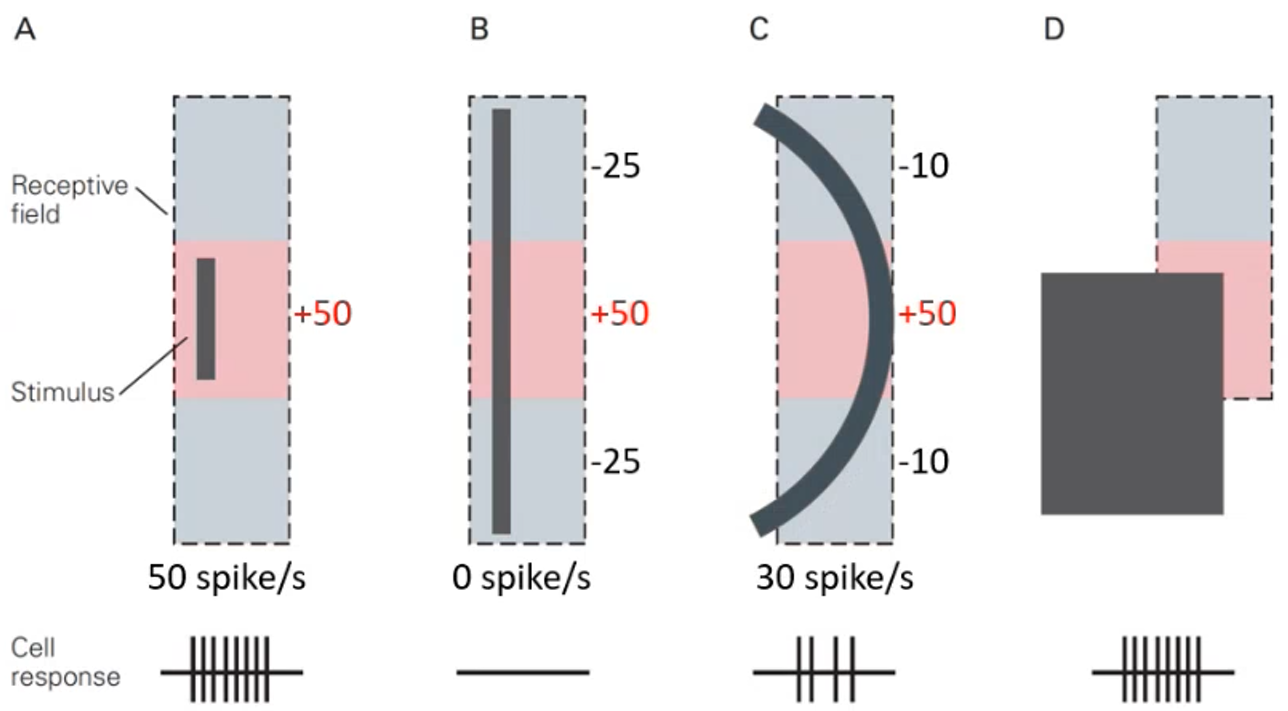
\includegraphics[width=0.5\linewidth]{./img/end_stopped_cell.png}
    \caption{End-stopped cell with a vertical preferred orientation}
\end{figure}


\subsection{Ice cube model}

Each 1 mm of the visual cortex can be modeled through an ice cube module 
that has all the neurons for decoding all the information (e.g. color, direction, \dots) in a specific location of the visual scene (i.e. each cube is a block of filters).

\begin{figure}[H]
    \centering
    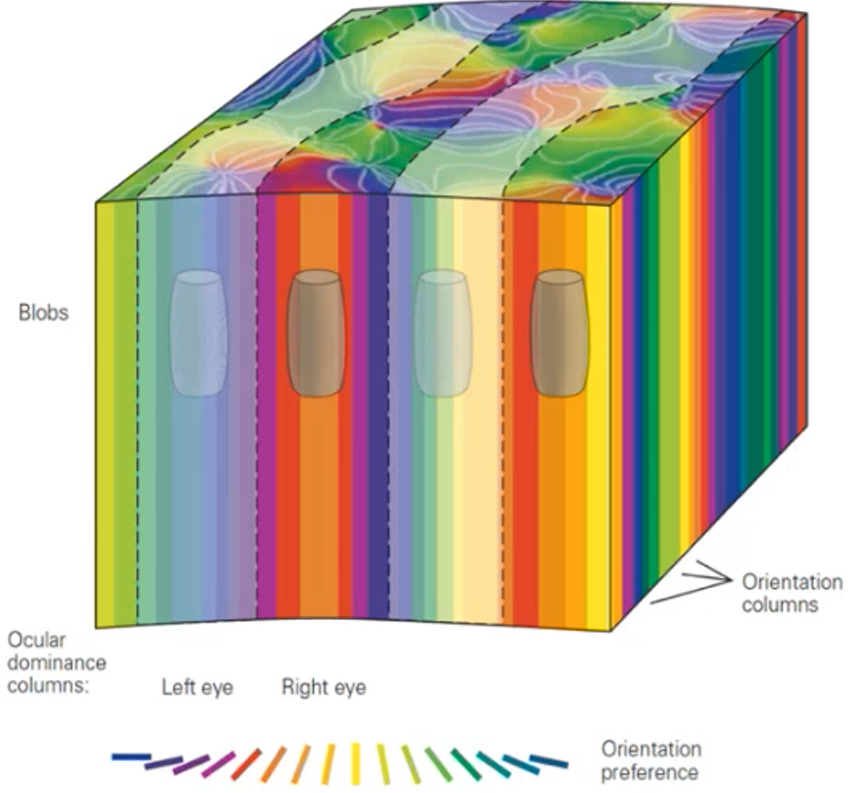
\includegraphics[width=0.3\linewidth]{./img/ice_cube.png}
\end{figure}



\section{Extrastriate visual areas}

\begin{description}
    \item[Extrastriate visual areas] Areas outside the primary visual cortex (V1).
        They are responsible for the actual object recognition task.
\end{description}

\begin{figure}[H]
    \centering
    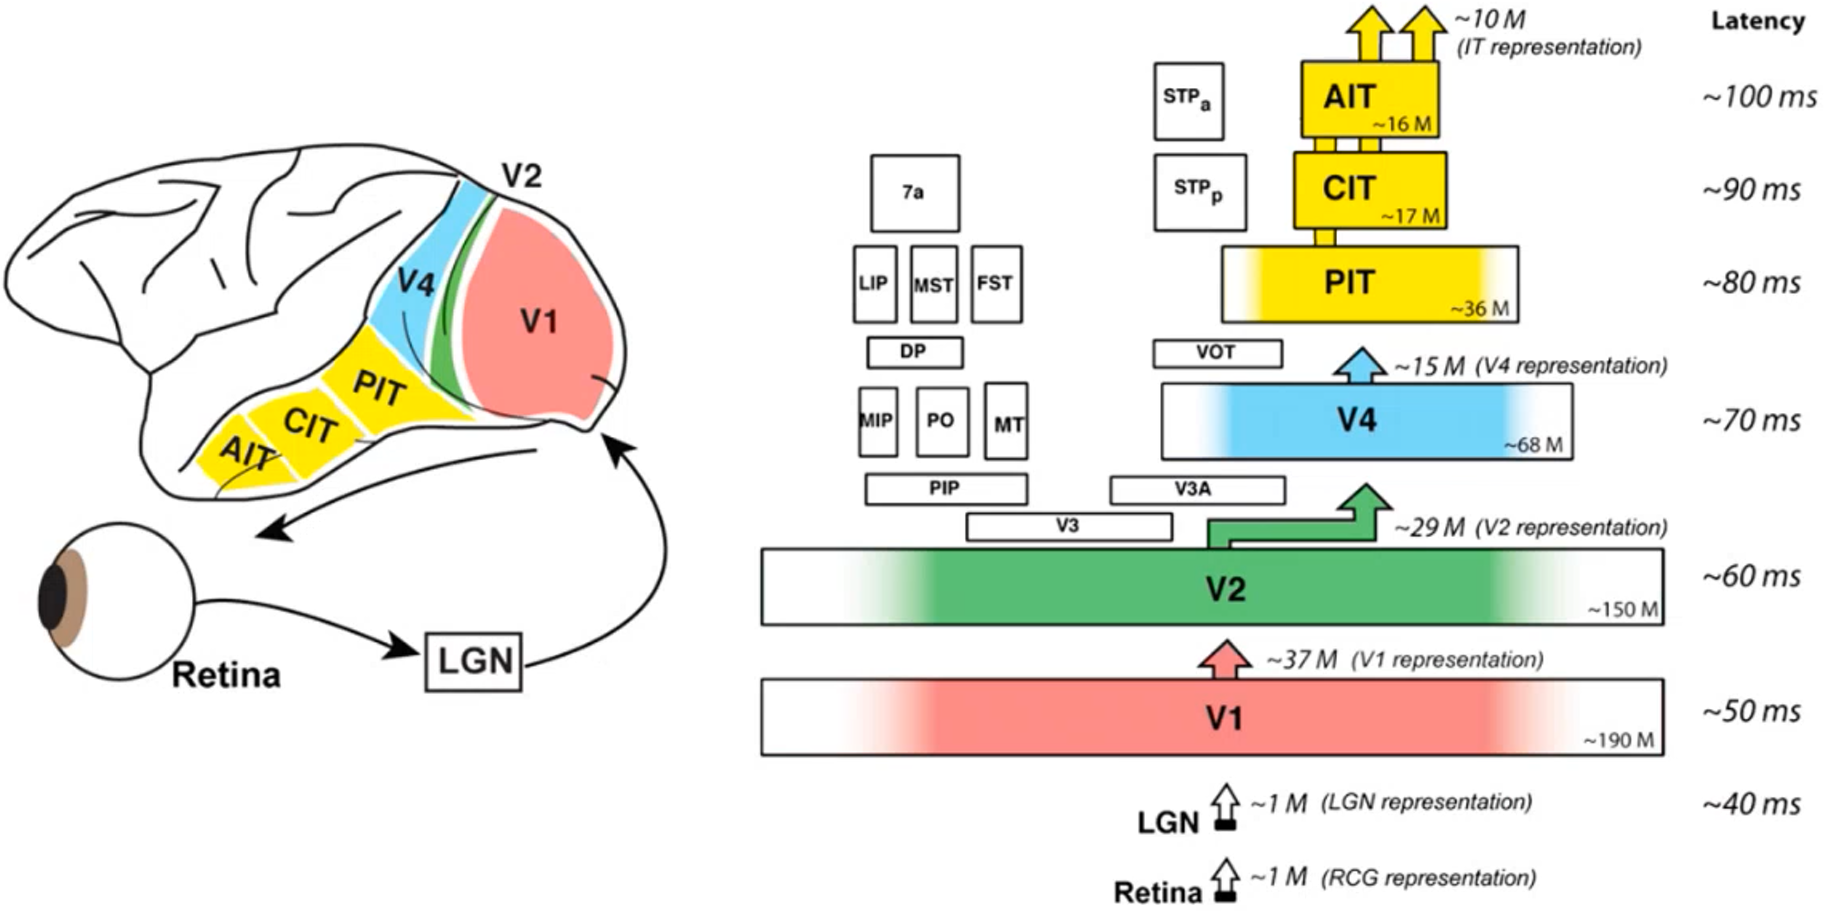
\includegraphics[width=0.55\linewidth]{./img/ventral_pathway.png}
    \caption{Ventral pathway}
\end{figure}


\begin{description}
    \item[Visual object] \marginnote{Visual object}
        Set of visual features (e.g. color, direction, orientation, \dots) perceptually grouped into discrete units.

    \item[Visual recognition]
        Ability to assign a verbal label to objects in the visual scene.
        \begin{description}
            \item[Identification] \marginnote{Identification} 
                Recognize the object at its individual level.
            \item[Categorization] \marginnote{Categorization} 
                Recognize the object as part of a more general category.
        \end{description}

        \begin{remark}
            In humans, categorization is easier than identification.
            Stimuli originating from distinct objects are usually treated as the same on the basis of past experience.

            % This behavior is motivated from a survival point of view.
        \end{remark}
\end{description}

\begin{figure}[H]
    \centering
    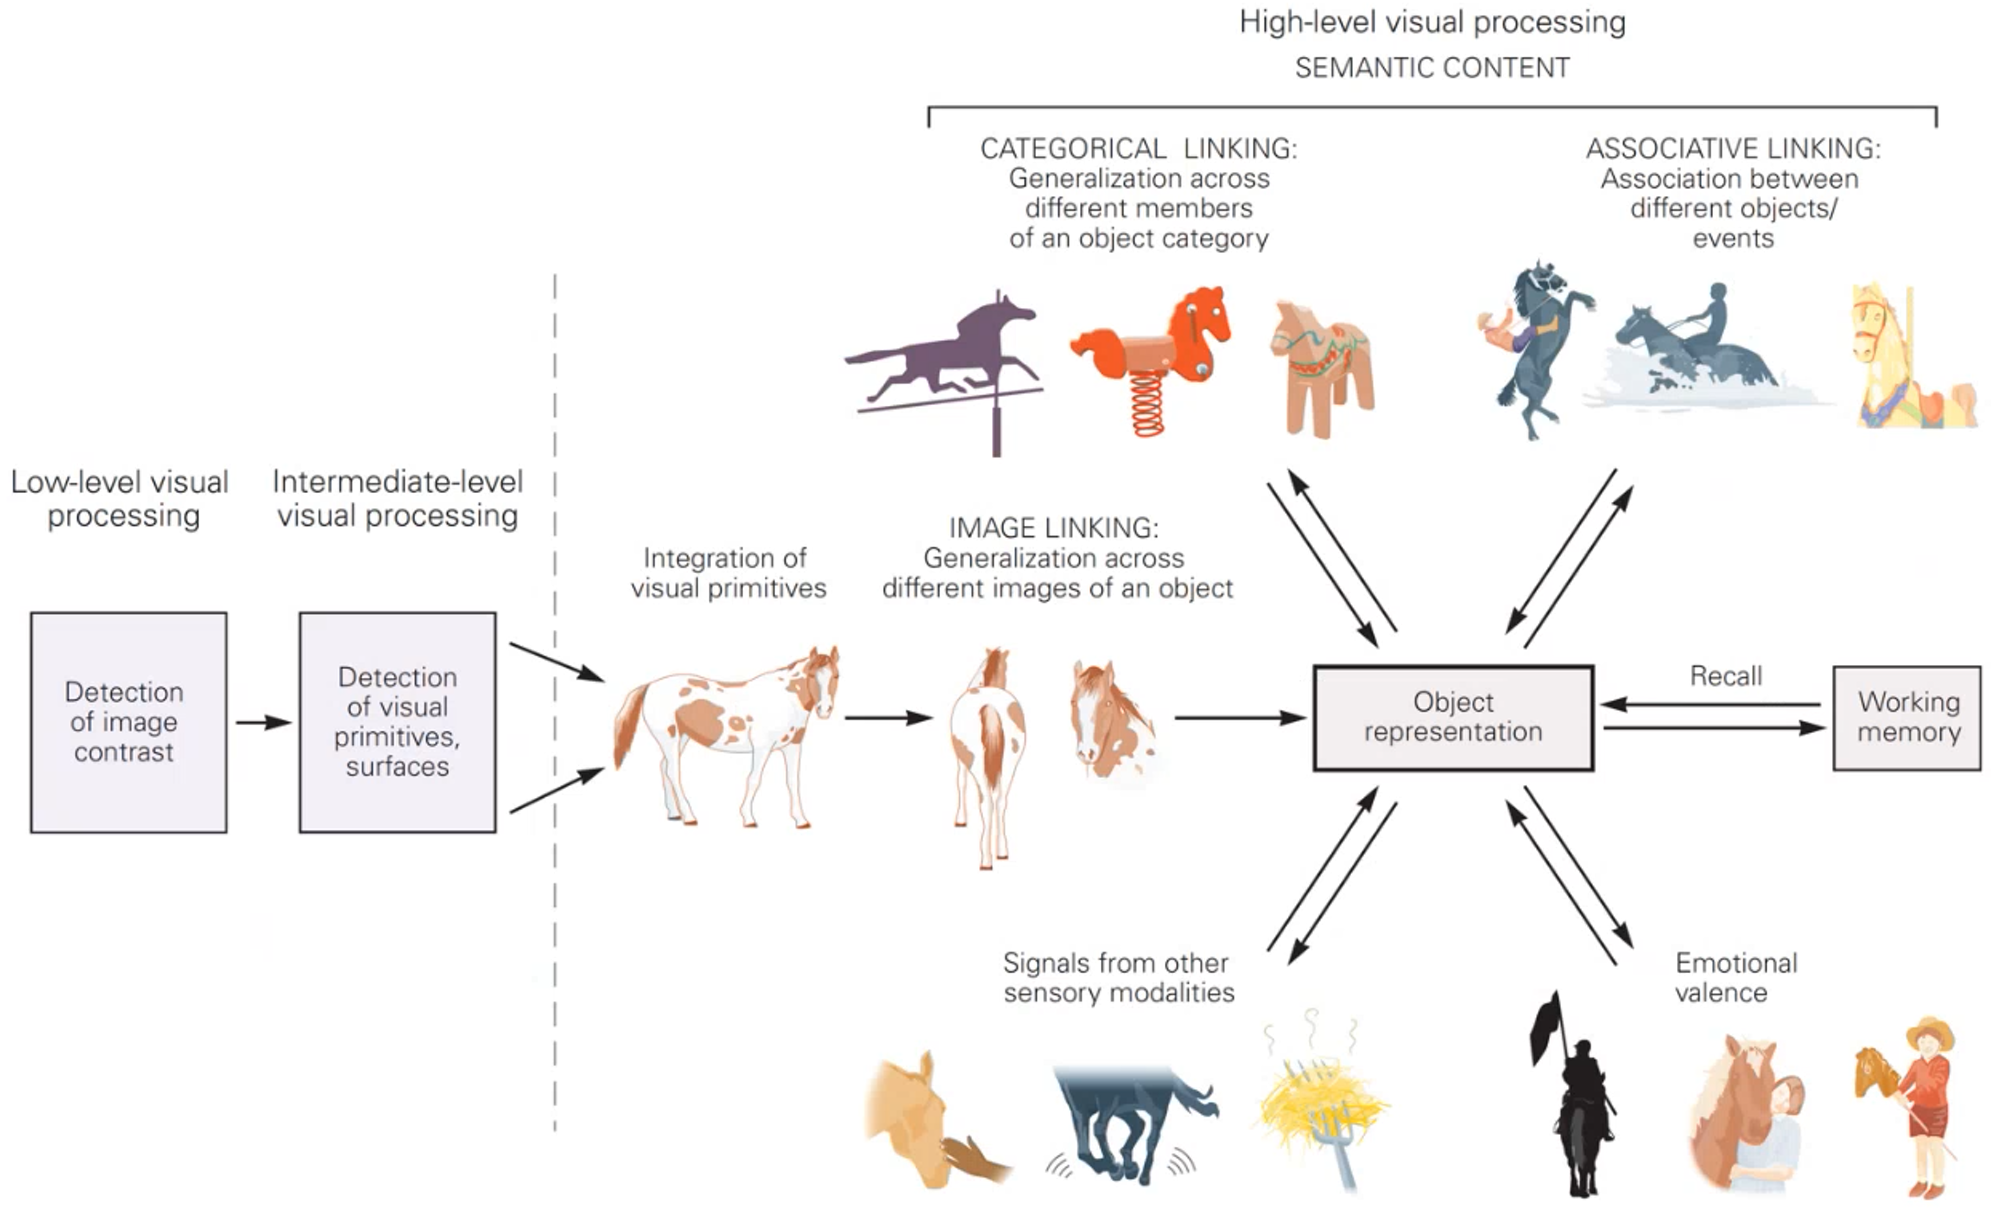
\includegraphics[width=0.7\linewidth]{./img/object_recognition.png}
    \caption{Processes that start after an object has been recognized}
\end{figure}

\begin{remark}
    For survival reasons, after an object has been recognized, 
    its emotional valence is usually the first thing that is retrieved to determine if the object is dangerous.
\end{remark}


Object recognition requires both the following competing properties:
\begin{descriptionlist}
    \item[Selectivity] \marginnote{Selectivity}
        Different responses to distinct specific objects.

    \item[Consistency] \marginnote{Consistency}
        Similar responses to transformations (e.g. rotation) of the same object (generalization).
\end{descriptionlist}

\begin{description}
    \item[Core object recognition] \marginnote{Core object recognition}
        Ability to rapidly ($< 200$ ms) discriminate a given visual object from all the other possible objects.
        \begin{remark}
            Primates perform this task exceptionally well even if the object is transformed.
        \end{remark}

        \begin{remark}
            200 ms is the time required to move the eyes. Experiments on core object recognition don't want candidates to move their eyes.
            Moreover, it prevents feed-back processing from starting.
        \end{remark}
\end{description}


\subsection{Area V4}
\marginnote{Area V4}

Intermediate cortical area responsible for visual object recognition and visual attention.
It facilitates figure-ground segmentation of the visual scene enabling both bottom-up and top-down visual processes.


\subsection{Inferior temporal cortex (IT)}
\marginnote{Inferior temporal cortex (IT)}

Responsible for object perception and recognition.
It is divided into three areas:
\begin{itemize}
    \item Anterior IT (AIT).
    \item Central IT (CIT).
    \item Posterior IT (PIT).
\end{itemize}

\begin{remark}
    It takes approximately 100 ms for the signal to arrive from the retina to the IT.
\end{remark}

\begin{remark}
    The number of neurons decreases from the retina to the IT.
    V1 can be seen as the area that sees everything and decides what to further process.
\end{remark}

\begin{remark}
    Central IT and anterior IT do not show clear retinotopy.
    Posterior IT shows some sort of pattern.
\end{remark}

\begin{remark}
    Receptive field scales by a factor of $\sim 3$ after passing through each cortical area.
    \begin{figure}[H]
        \centering
        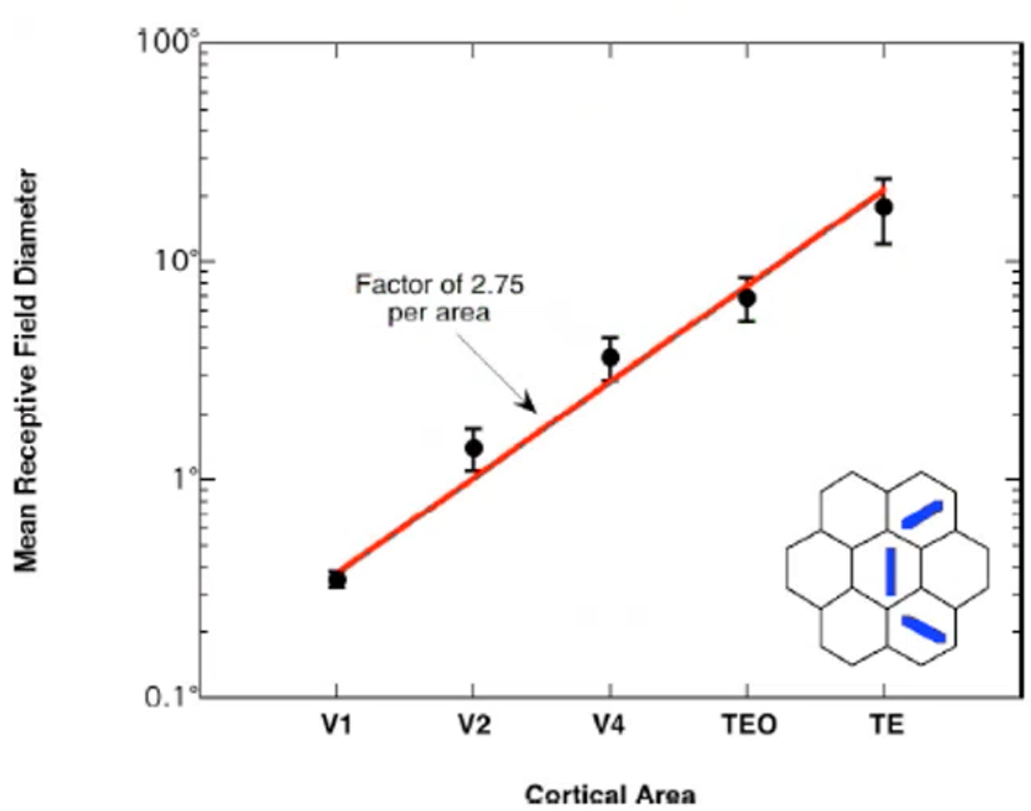
\includegraphics[width=0.4\linewidth]{./img/receptive_field_growth.png}
    \end{figure}
\end{remark}

\begin{remark}
    It is difficult to determine which stimuli trigger the neurons in the IT and
    what actual stimuli trigger the IT is still unclear.

    Generally, neurons in this area respond to complex stimuli, often biologically relevant objects (e.g. faces, hands, animals, \dots).
    
    \begin{figure}[H]
        \centering
        \begin{subfigure}{0.35\linewidth}
            \centering
            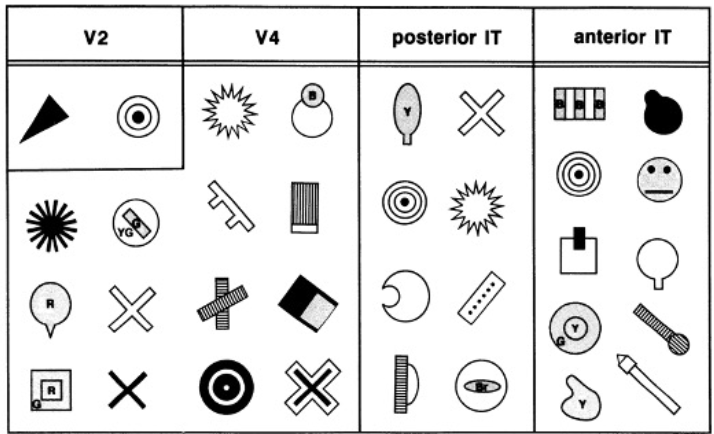
\includegraphics[width=0.95\linewidth]{./img/vision_complexity.png}
            \caption{Stimuli that trigger specific neurons of the ventral pathway}
        \end{subfigure}
        \begin{subfigure}{0.6\linewidth}
            \centering
            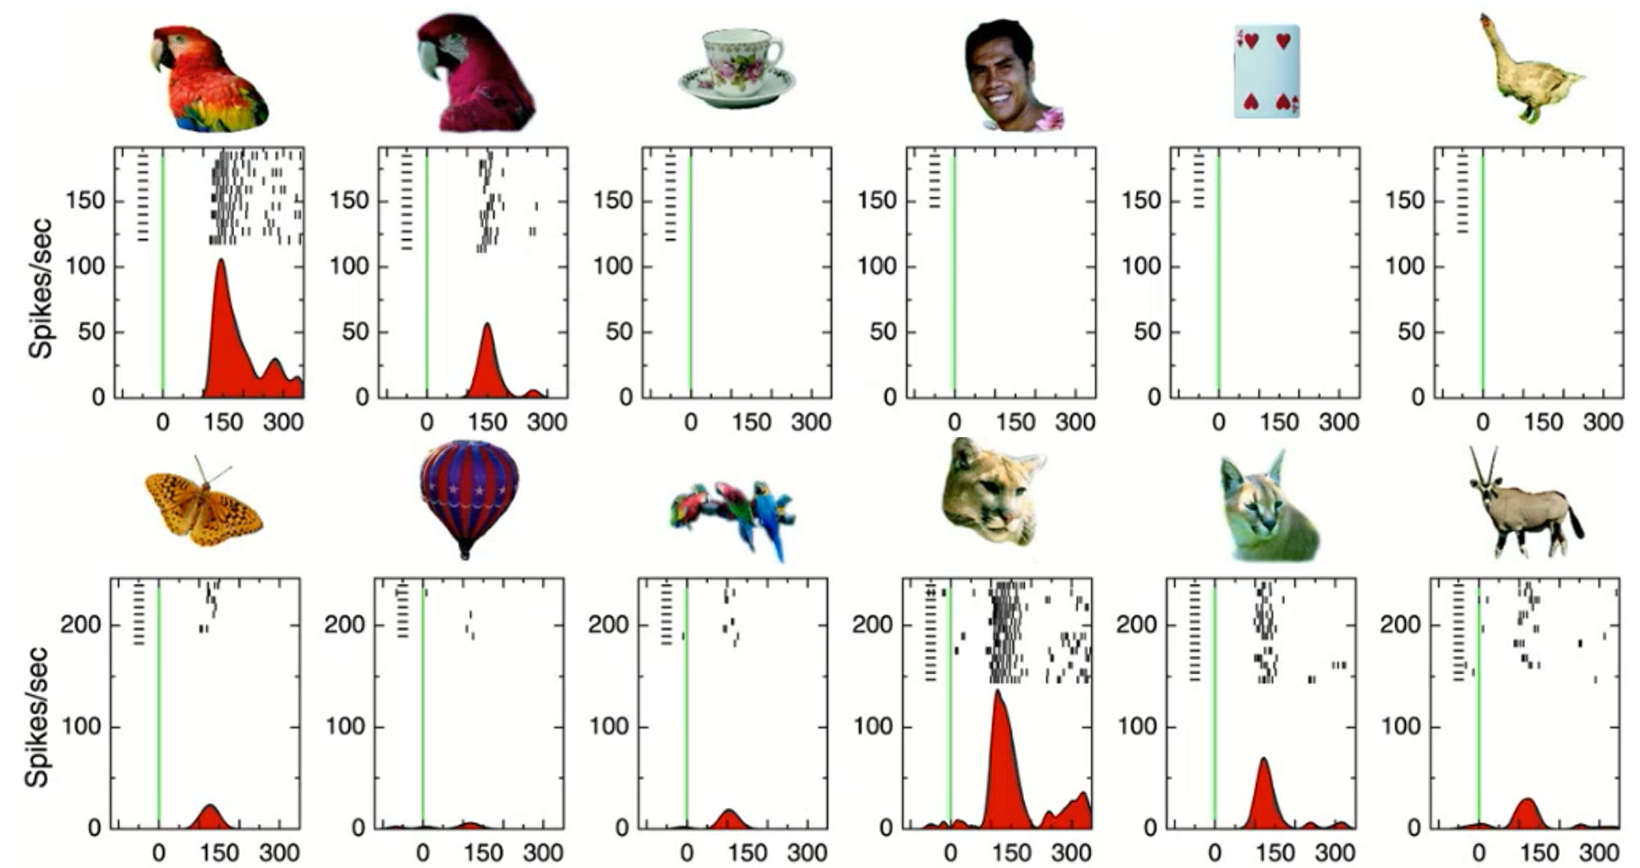
\includegraphics[width=0.95\linewidth]{./img/it_response.png}
            \caption{Responses of a specific IT neuron to different stimuli}
        \end{subfigure}
    \end{figure}
\end{remark}


\begin{casestudy}[IT neurons in monkeys]
    Several researchers observed that a group of IT neurons in monkeys respond selectively to faces.
    The response is stronger when the full face is visible and gets weaker if it is incomplete or malformed.
    \begin{figure}[H]
        \centering
        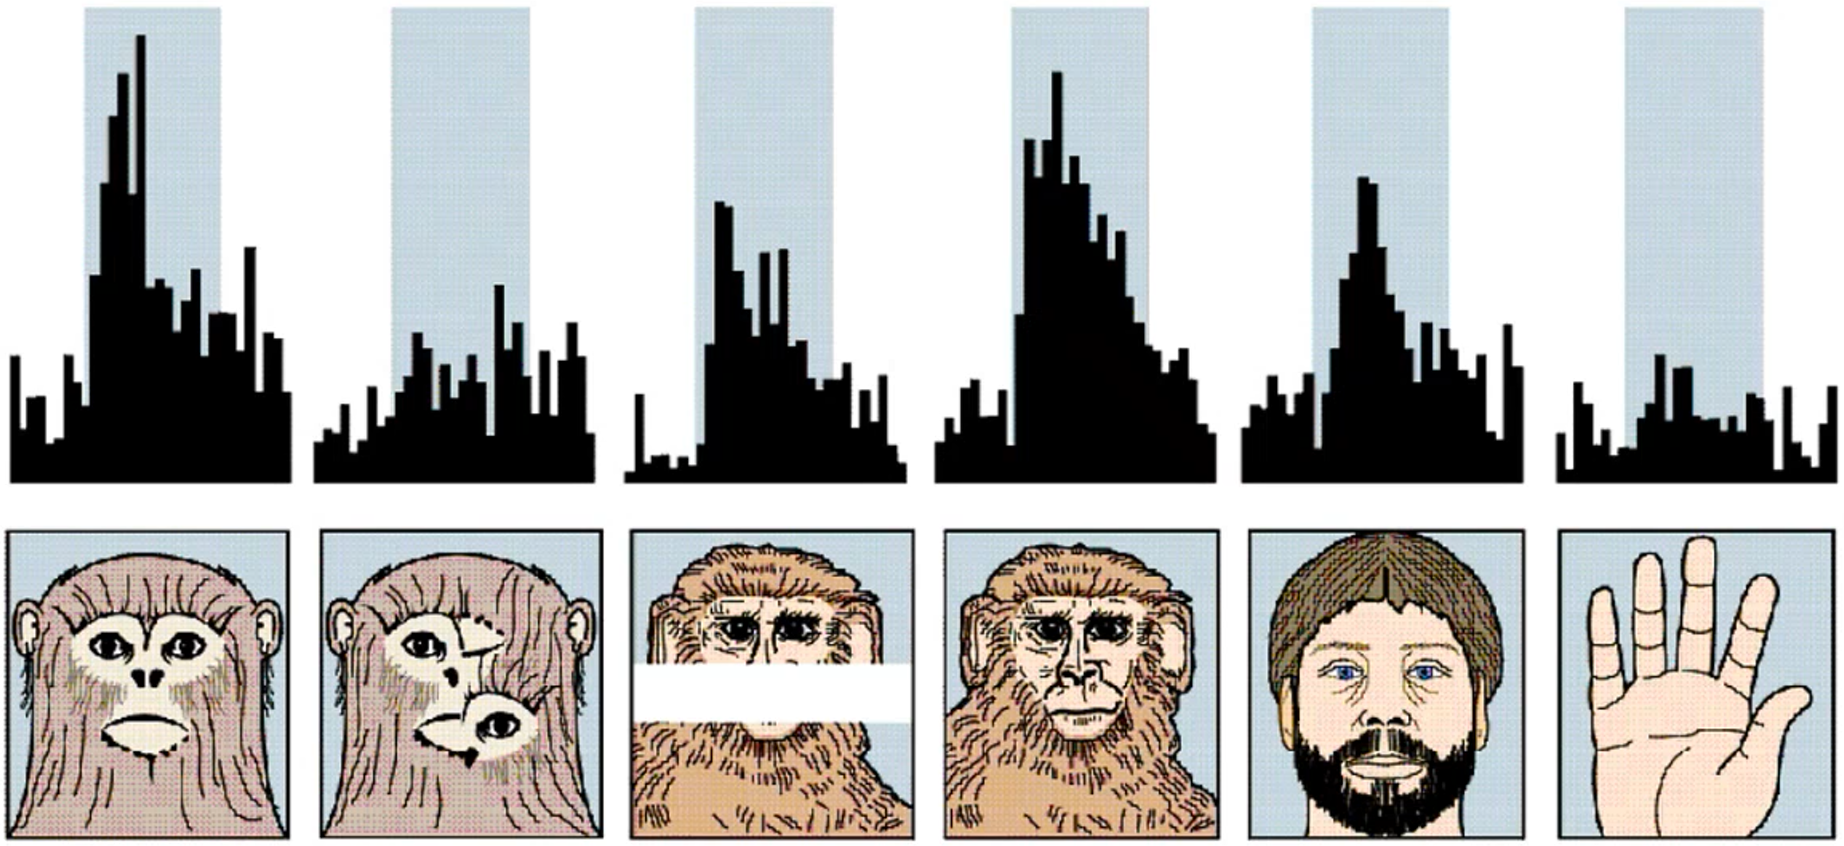
\includegraphics[width=0.4\linewidth]{./img/monkey_it_faces.png}
    \end{figure}

    It also has been observed that an IT neuron responds to hands presented at various perspectives and orientations.
    A decrease in response is visible when the hand gets smaller and it is clearly visible when a glove is presented.
    \begin{figure}[H]
        \centering
        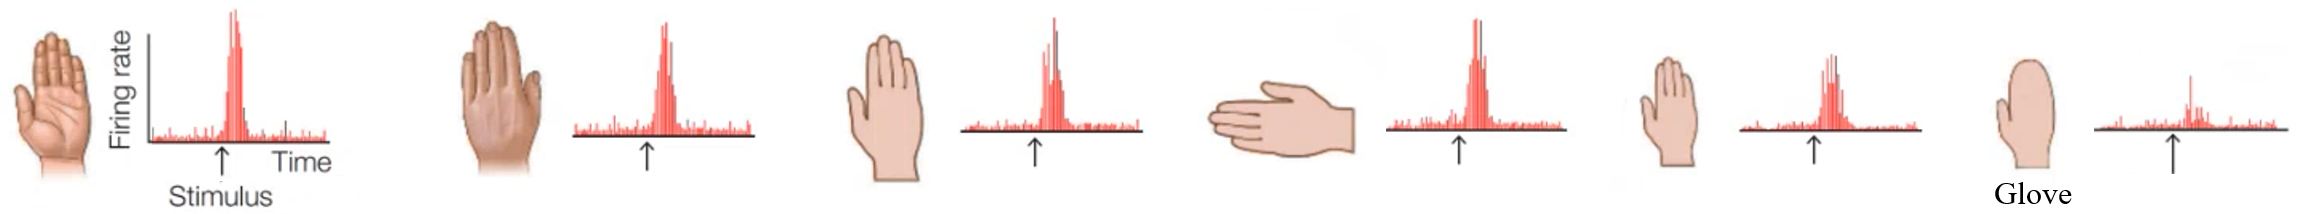
\includegraphics[width=0.95\linewidth]{./img/monkey_it_hands.png}
    \end{figure}
\end{casestudy}

\begin{casestudy}[IT neuron response to a melon]
    An IT neuron responds to a complex image of a melon.
    However, it has been shown that it also responds to simpler stimuli that represent the visual elements of the melon.

    \begin{figure}[H]
        \centering
        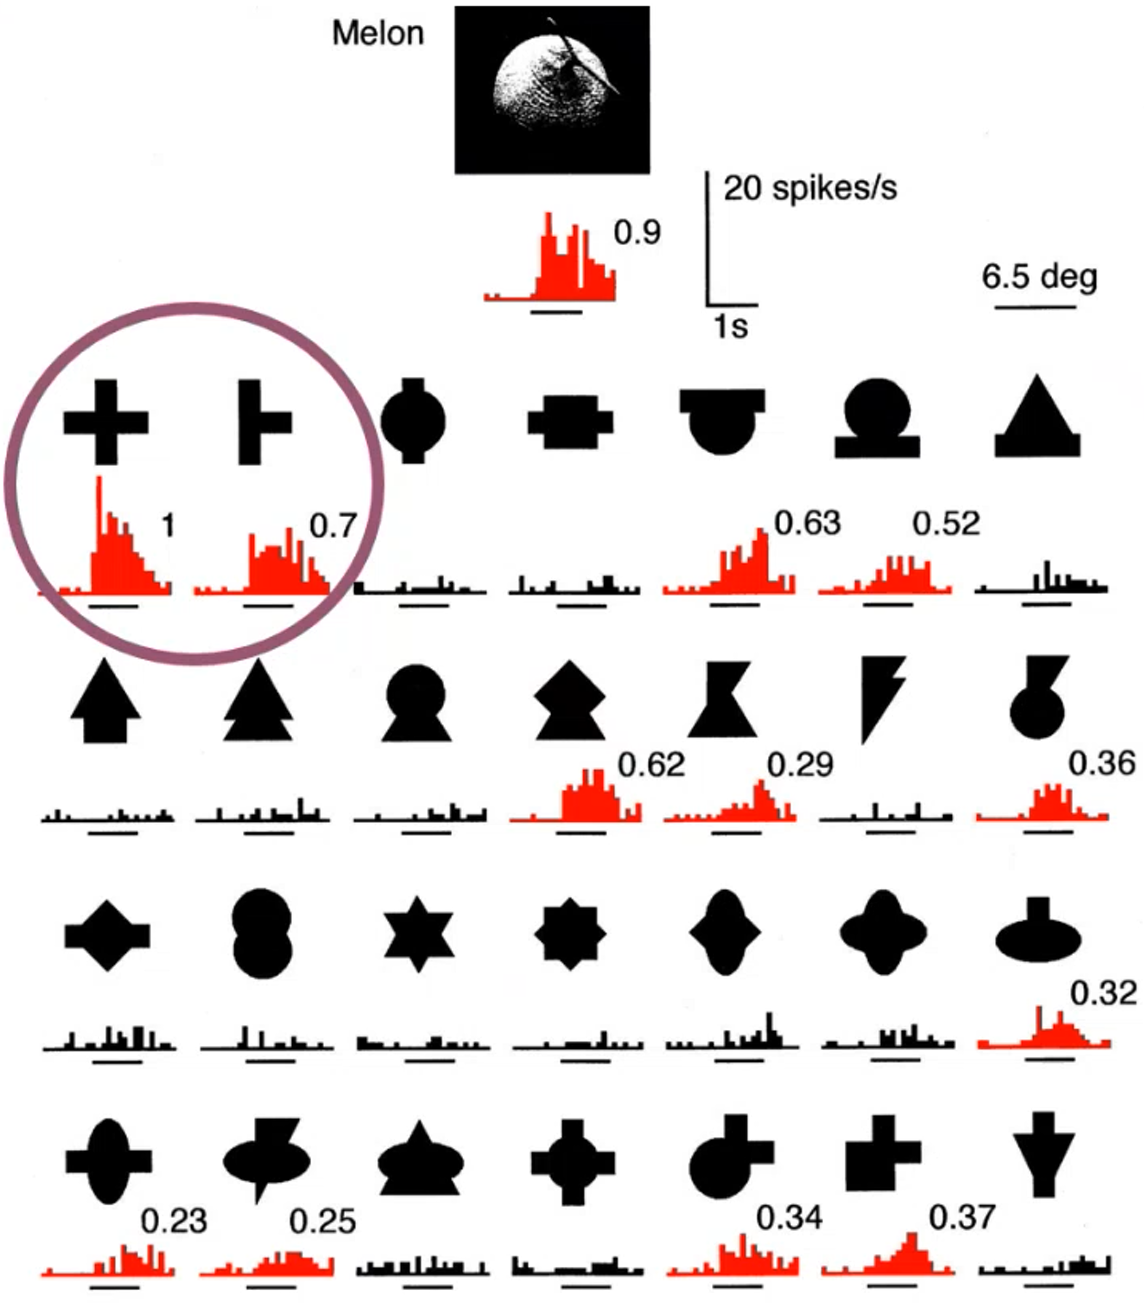
\includegraphics[width=0.4\linewidth]{./img/it_melon.png}
    \end{figure}
\end{casestudy}

\begin{description}
    \item[View-dependent unit] \marginnote{View-dependent unit}
        The majority of IT neurons are view-dependent and respond only to objects at specific points of view.

    \item[View-invariant unit] \marginnote{View-invariant unit}
        10\% of IT neurons are view-invariant and respond regardless of the position of the observer.
\end{description}

\begin{figure}[H]
    \centering
    \begin{subfigure}{0.48\linewidth}
        \centering
        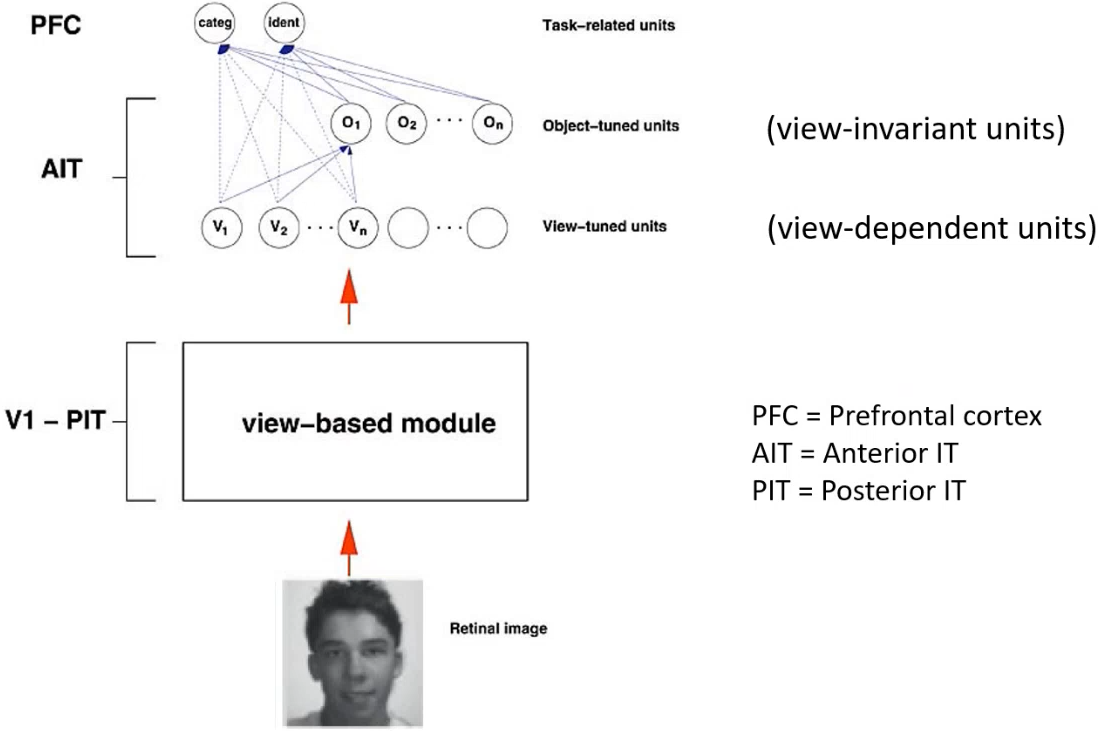
\includegraphics[width=0.95\linewidth]{./img/object_recognition_process.png}
    \end{subfigure}
    \begin{subfigure}{0.48\linewidth}
        \centering
        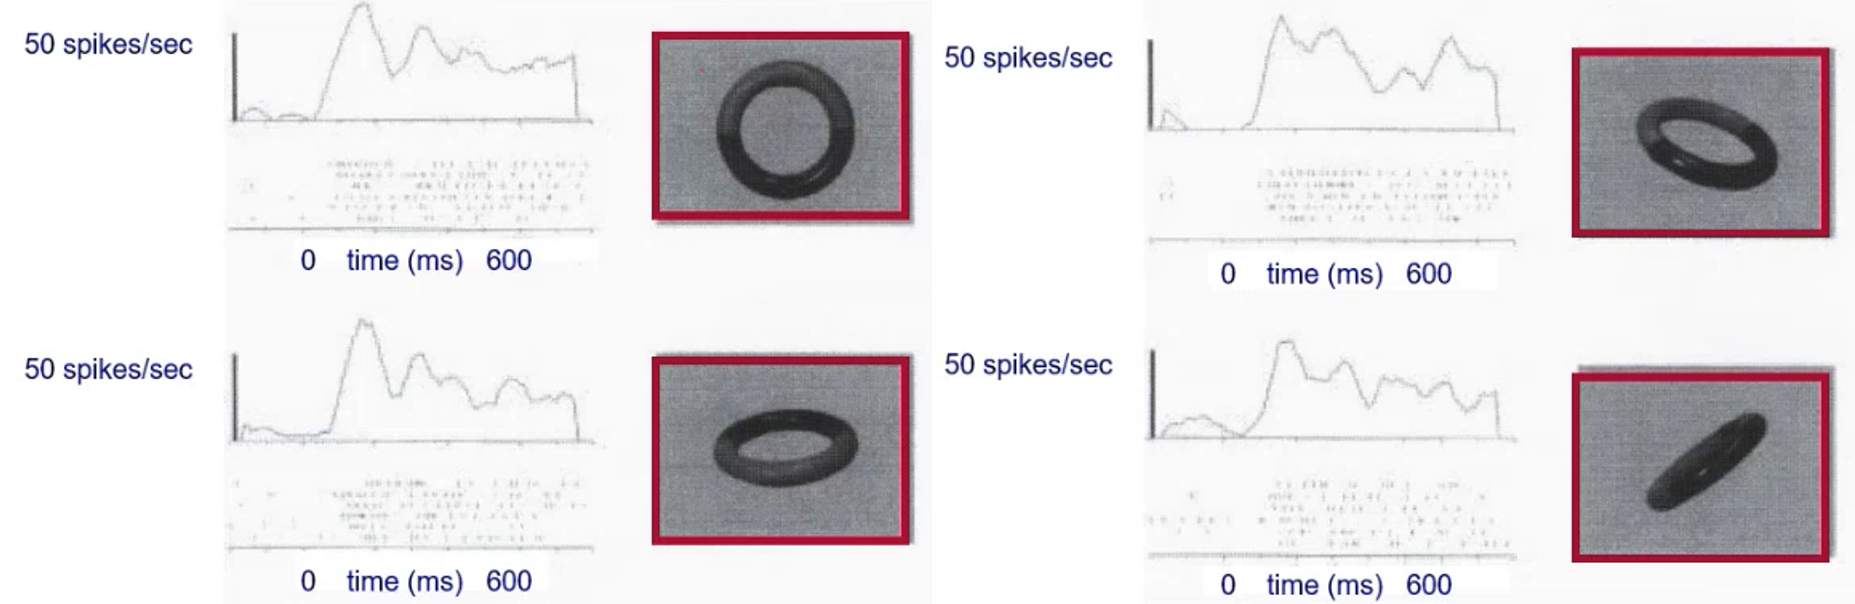
\includegraphics[width=0.95\linewidth]{./img/it_view_independent_response.png}
        \caption{View-invariant unit}
    \end{subfigure}
\end{figure}


\begin{description}
    \item[Gnostic unit] \marginnote{Gnostic unit}
        Neuron in the object detection hierarchy that gets activated by complex stimuli (i.e. objects with a meaning).
\end{description}

\begin{casestudy}[Jennifer Aniston cell]
    An IT neuron of a human patient only responded to pictures of Jennifer Aniston or to its written name.
    \begin{figure}[H]
        \centering
        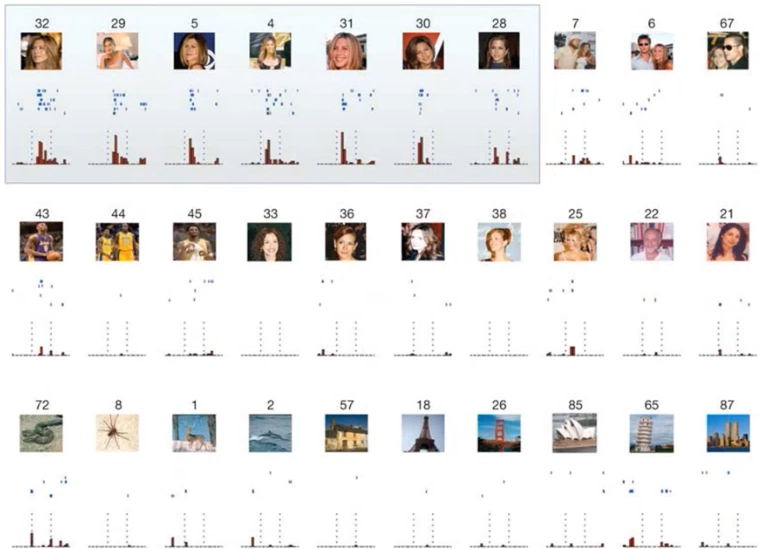
\includegraphics[width=0.5\linewidth]{./img/aniston_cell.png}
    \end{figure}
\end{casestudy}



\subsection{Local vs distributed coding}


\begin{description}
    \item[Local coding hypothesis] \marginnote{Local coding hypothesis}
        IT neurons are gnostic units that are activated only when a particular object is recognized.

    \item[Distributed coding hypothesis] \marginnote{Distributed coding hypothesis}
        Recognition is due to the activation of multiple IT neurons.
        \begin{remark}
            This is the most plausible hypothesis.
        \end{remark}
\end{description}


\begin{casestudy}[Neurons in vector space]
    The response of a population of neurons can be represented in a vector space.
    It is expected that transformations of the same object produce representations that lie on the same manifold. 

    In the first stages of vision processing, various manifolds are tangled.
    Object recognition through the visual cortex aims to untangle the representations of the objects.

    \begin{figure}[H]
        \centering
        \begin{subfigure}{0.48\linewidth}
            \centering
            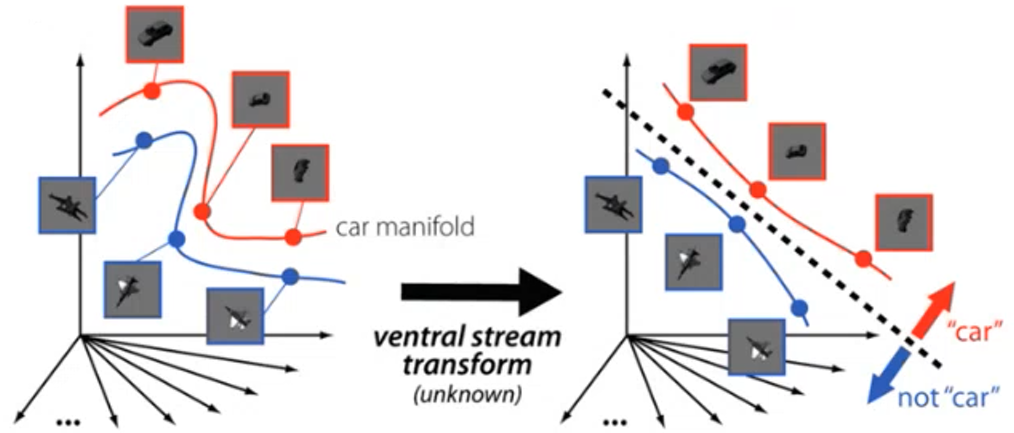
\includegraphics[width=0.95\linewidth]{./img/tangled_vectors.png}
        \end{subfigure}
        \begin{subfigure}{0.48\linewidth}
            \centering
            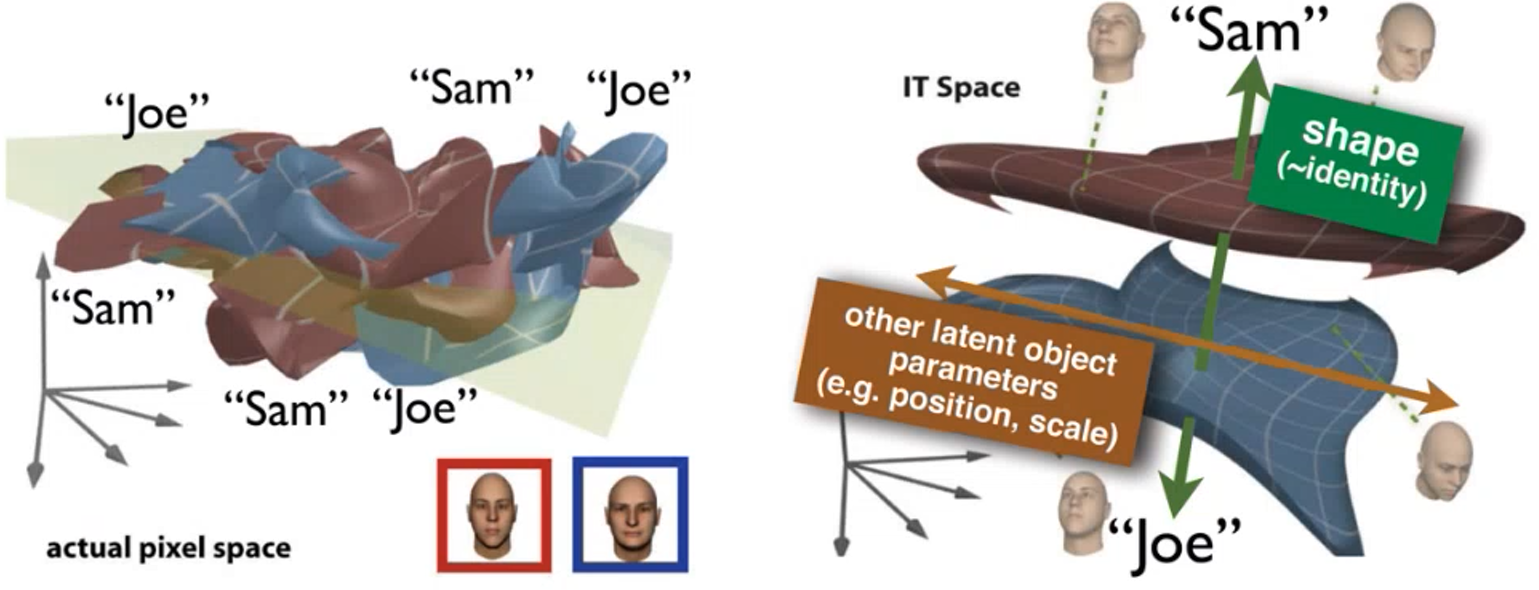
\includegraphics[width=0.95\linewidth]{./img/tangled_joe_sam.png}
        \end{subfigure}
    \end{figure}
\end{casestudy}


\begin{casestudy}[Classifier from monkey neurons \cite{vision_monkey_svm}]
    An animal maintains fixation at the center of a screen on which images of different categories are presented very quickly (100 ms + 100 ms pause)
    at different scales and positions.

    The responses of IT neurons are taken with some offset after the stimulus (to give them time to reach the IT)
    and converted into vector form to train one binary classifier (SVM) for each category (one-vs-all).

    Once trained, testing was done on new stimuli.
    Results show that the performance increases linearly with the logarithm of the number of sites (measured neurons).
    It can be concluded that:
    \begin{itemize}
        \item Categorization is easier than identification.
        \item The distributed coding hypothesis is more likely.
    \end{itemize}

    \begin{figure}[H]
        \centering
        \begin{subfigure}{0.3\linewidth}
            \centering
            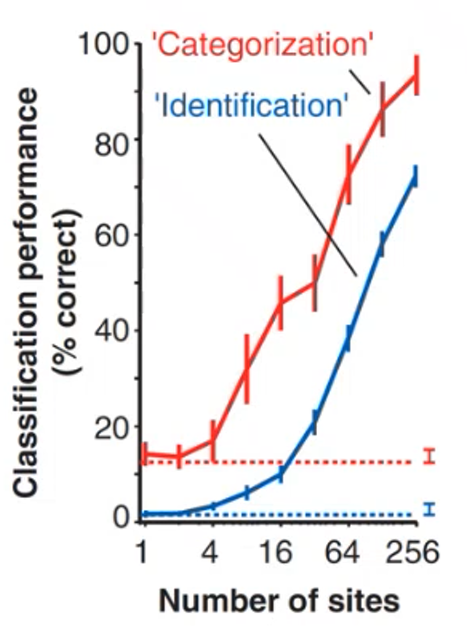
\includegraphics[width=0.65\linewidth]{./img/monkey_svm_results.png}
        \end{subfigure}
        \begin{subfigure}{0.6\linewidth}
            \centering
            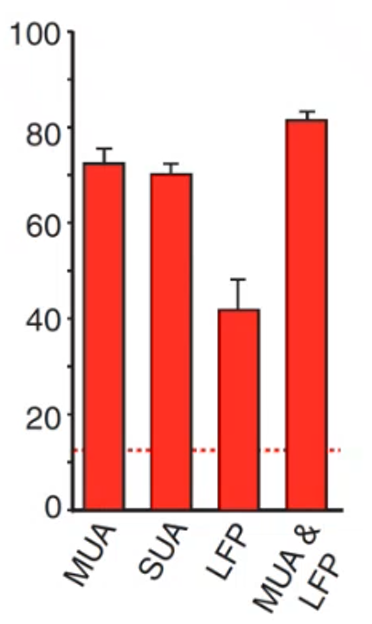
\includegraphics[width=0.25\linewidth]{./img/monkey_svm_results2.png}
            \caption{Accuracy on multiple units (MUA), a single unit (SUA) and readings made on the cortex, not inside (LFP)}
        \end{subfigure}
    \end{figure}

    Time-wise, it has been observed that:
    \begin{itemize}
        \item Performance gets worse if the measurement of the neurons spans for too long 
            (no explanation was given in the original paper, probably noise is added up to the signal for longer measurements).
        \item The best offset from the stimulus onset at which the measures of the IT neurons should be taken is 125 ms.
    \end{itemize}

    \begin{figure}[H]
        \centering
        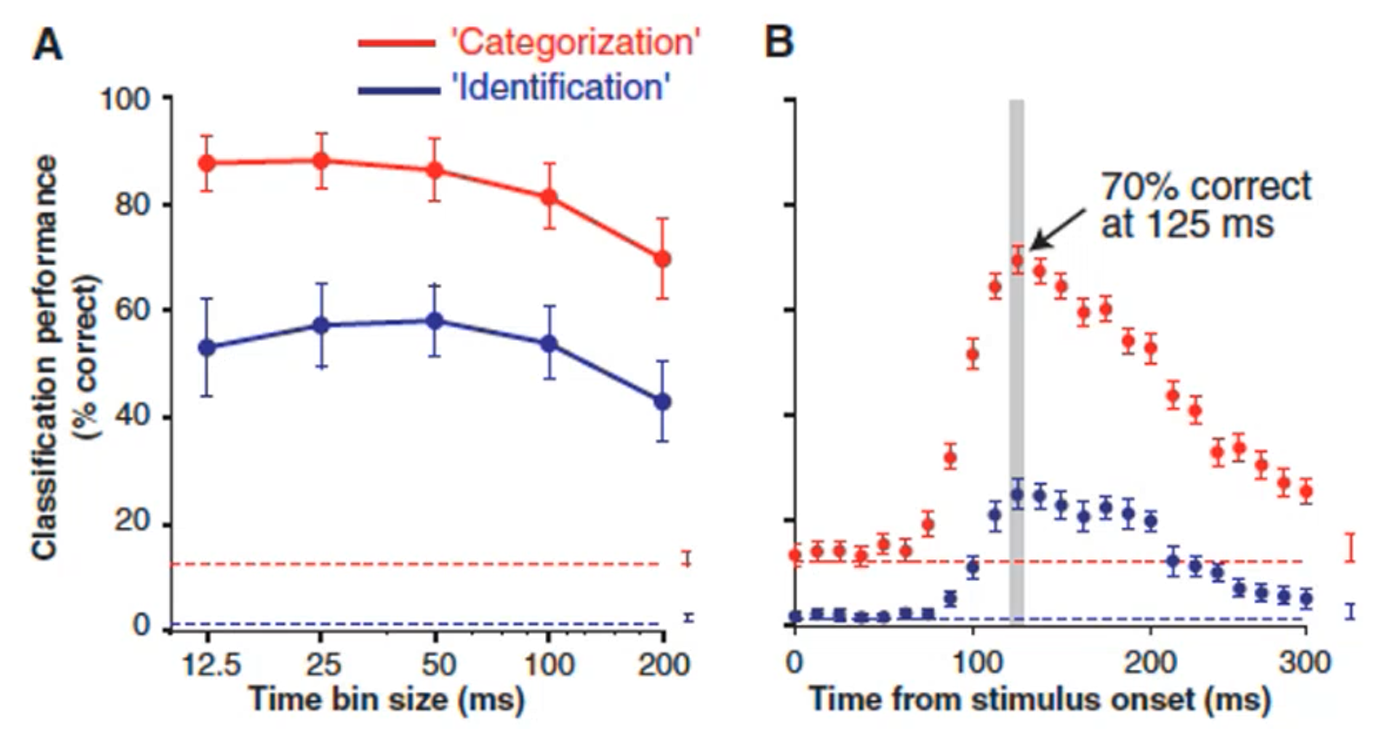
\includegraphics[width=0.5\linewidth]{./img/monkey_svm_time.png}
    \end{figure}

    It has also been observed that the visual ventral pathway, which is responsible for object recognition, also encodes information on the size of the objects.
    This is not strictly useful for recognition, but a machine learning algorithm is able to extract this information from the neural readings.
    This hints at the fact that the ventral pathway also contributes to identifying the location and size of the objects.
\end{casestudy}


\begin{casestudy}[Artificial neural network to predict neuronal activity \cite{vision_monkey_hcnn}]
    Different neural networks are independently trained on the task of image recognition.
    Then, the resulting networks are compared to the neuronal activity of the brain.

    The network should have the following properties:
    \begin{itemize}
        \item Provide information useful to support behavioral tasks (i.e. act as the IT neurons).
        \item Layers of the network should have a corresponding area on the ventral pathway (mappable).
        \item It should be able to predict the activation of single and groups of biological neurons (neurally predictive).
    \end{itemize}

    \begin{descriptionlist}
        \item[Dataset] 
            A set of images is divided into two sets:
            \begin{descriptionlist}
                \item[Train set] To train the neural networks.
                \item[Test set] To collect neuronal data and evaluate the neural networks.
            \end{descriptionlist}

            Images have different levels of difficulty (low to high variation) and are presented on random backgrounds.
            \begin{figure}[H]
                \centering
                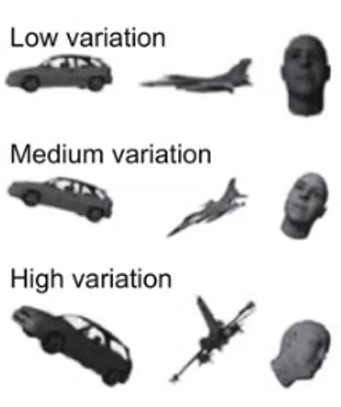
\includegraphics[width=0.2\linewidth]{./img/vision_nn_difficulty.png}
            \end{figure}


        \item[Neuronal data]
            Neuronal data are collected from the area V4 and IT in two macaque monkeys.
            They are tasked to maintain fixation at the center of a screen on which images are presented for 100 ms followed by a 100 ms blank screen.

            For each stimulus, the firing rate is obtained as the average of the number of spikes in the interval 70 ms - 170 ms after the stimulus onset.


        \item[Neural network training] 
            Hierarchical convolutional neural networks (HCNN) are used for the experiments.
            They are composed of linear-nonlinear layers that do the following:
            \begin{enumerate}
                \item Filtering through linear operations of the input stimulus (i.e. convolutions).
                \item Activation through a rectified linear threshold or sigmoid.
                \item Mean or maximum pooling as nonlinear aggregation operation.
                \item Divisive normalization to output a standard range.
            \end{enumerate}
            \begin{figure}[H]
                \centering
                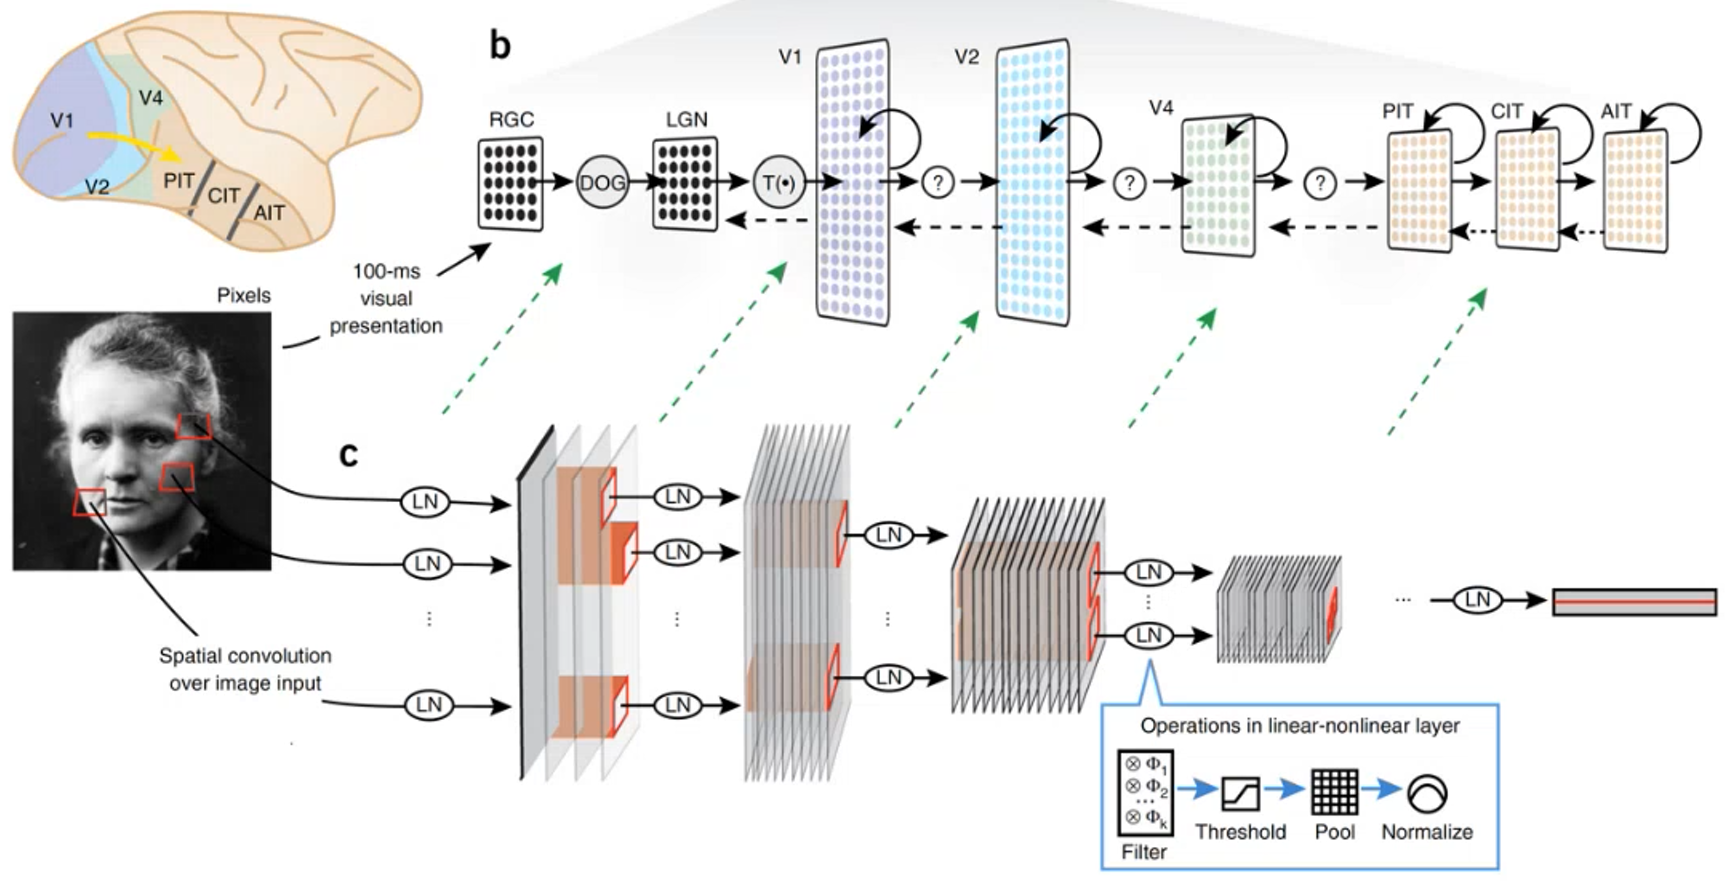
\includegraphics[width=0.7\linewidth]{./img/vision_nn_network.png}
            \end{figure}

            The HCNNs have a depth of 3 or fewer layers and are trained independently from the neuronal measurements.
            For evaluation, models are divided into groups following three different criteria:
            \begin{itemize}
                \item Random sampling.
                \item Selection of models with the highest performance on the high-variation images.
                \item Selection of models with the highest IT neural predictivity.
            \end{itemize}

            Resulting HCNNs are also used to create a new high-performance architecture through hierarchical modular optimization (HMO)
            by selecting the best-performing modules from the trained networks (as each layer is modular).


        \item[Evaluation method]
            Evaluation is done using the following approach:
            \begin{itemize}
                \item Object recognition performances are assessed using SVM classifiers:
                    \begin{itemize}
                        \item For neural networks, the output features of a stimulus are obtained from the activations at the top layers.
                        \item For neuronal readings, the output features of a stimulus are obtained by converting the firing rates into vector form.
                    \end{itemize}
                
                \item To measure the ability of a neural network to predict the activity of a neuron,
                    a partial least squares regression model is used to find a combination of weights at the top layers of the network
                    that best fits, using as metric the coefficient of determination ($R^2$), the activity of the neuron on a random subset of test images.

                \item An ideal observer is used as a baseline.
                    It has all the categorical information to make correct predictions but it does not use a layered approach.
            \end{itemize}


        \item[Results]
            It has been observed that:
            \begin{itemize}
                \item The HMO model has human-like performances.
                    \begin{figure}[H]
                        \centering
                        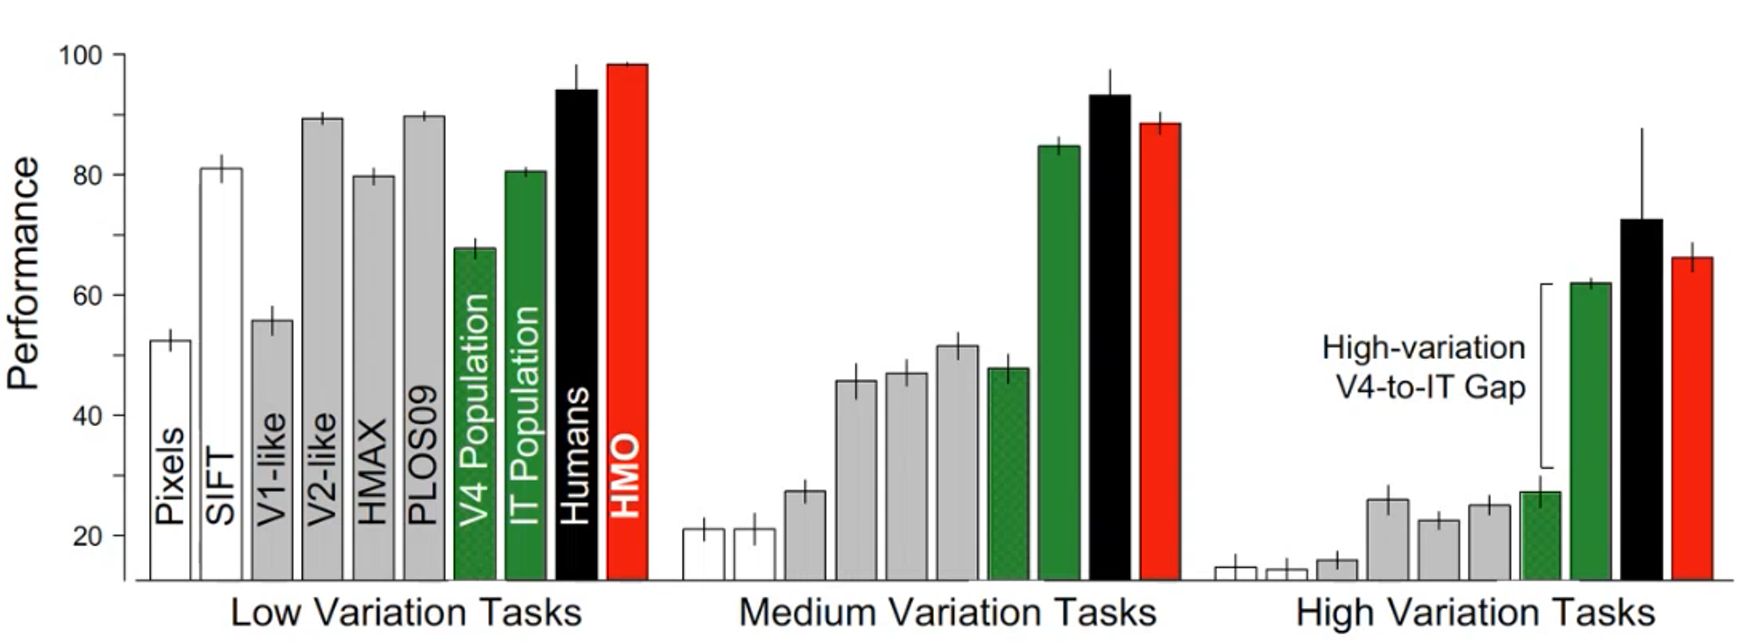
\includegraphics[width=0.7\linewidth]{./img/vision_nn_performance_hmo.png}
                    \end{figure}

                \item The higher the categorization accuracy, the better the model can explain the IT.
                    
                    Moreover, forcefully fitting a network to predict IT as the main task 
                    predicts the neuronal activity worse than using a model with high categorization accuracy.

                    \begin{figure}[H]
                        \centering
                        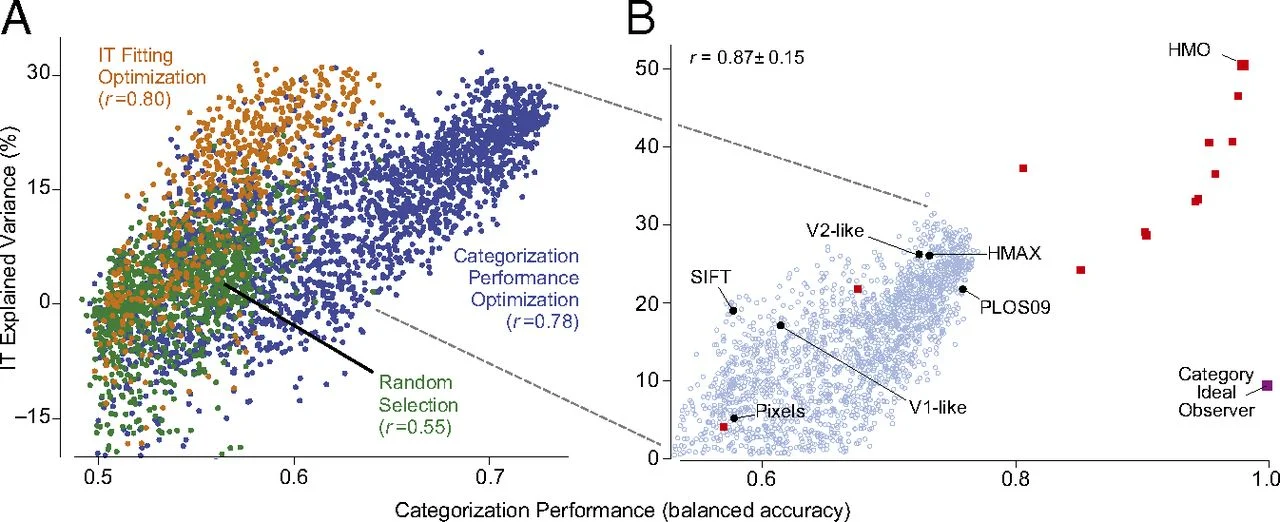
\includegraphics[width=0.7\linewidth]{./img/vision_nn_neural_prediction.png}
                    \end{figure}

                \item None of the parameters of the neural networks can independently predict the IT better than performance (i.e. the network as a whole).
                    \begin{figure}[H]
                        \centering
                        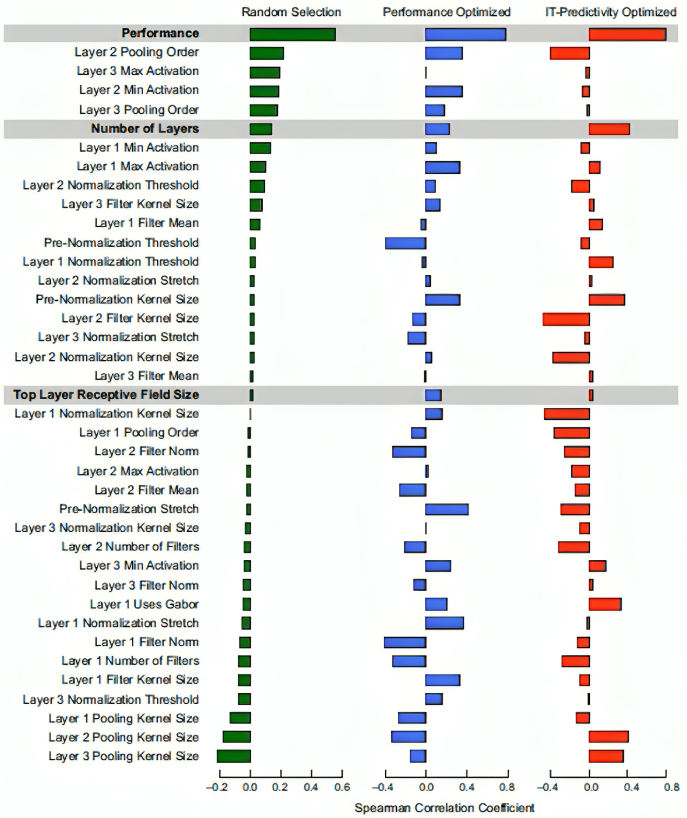
\includegraphics[width=0.5\linewidth]{./img/vision_nn_params_prediction.png}
                    \end{figure}

                \item Higher levels of the HMO model yield good prediction capabilities of IT and V4 neurons.
                    More specifically:
                    \begin{itemize}
                        \item The fourth (last) layer of the HMO model predicts well the IT.
                        \item The third layer of the HMO model predicts well the area V4.
                    \end{itemize}
                    \begin{figure}[H]
                        \centering
                        \begin{subfigure}{0.6\linewidth}
                            \centering
                            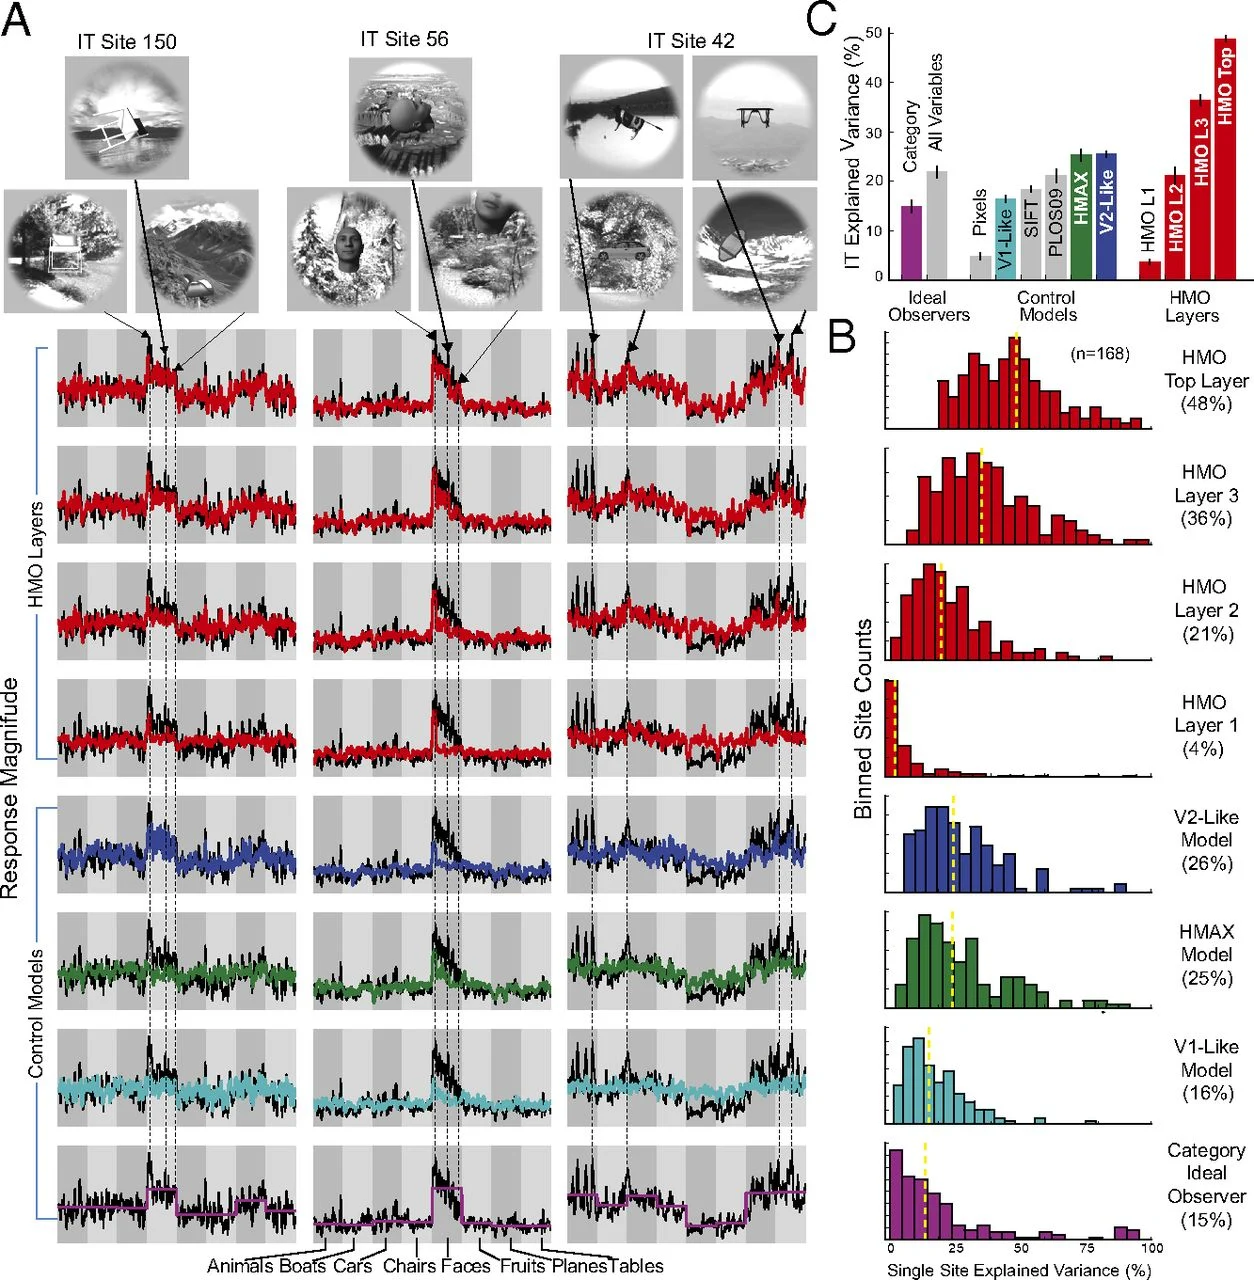
\includegraphics[width=\linewidth]{./img/vision_nn_prediction_it.png}
                            \caption{Results on IT}
                        \end{subfigure}
                        \begin{subfigure}{0.38\linewidth}
                            \centering
                            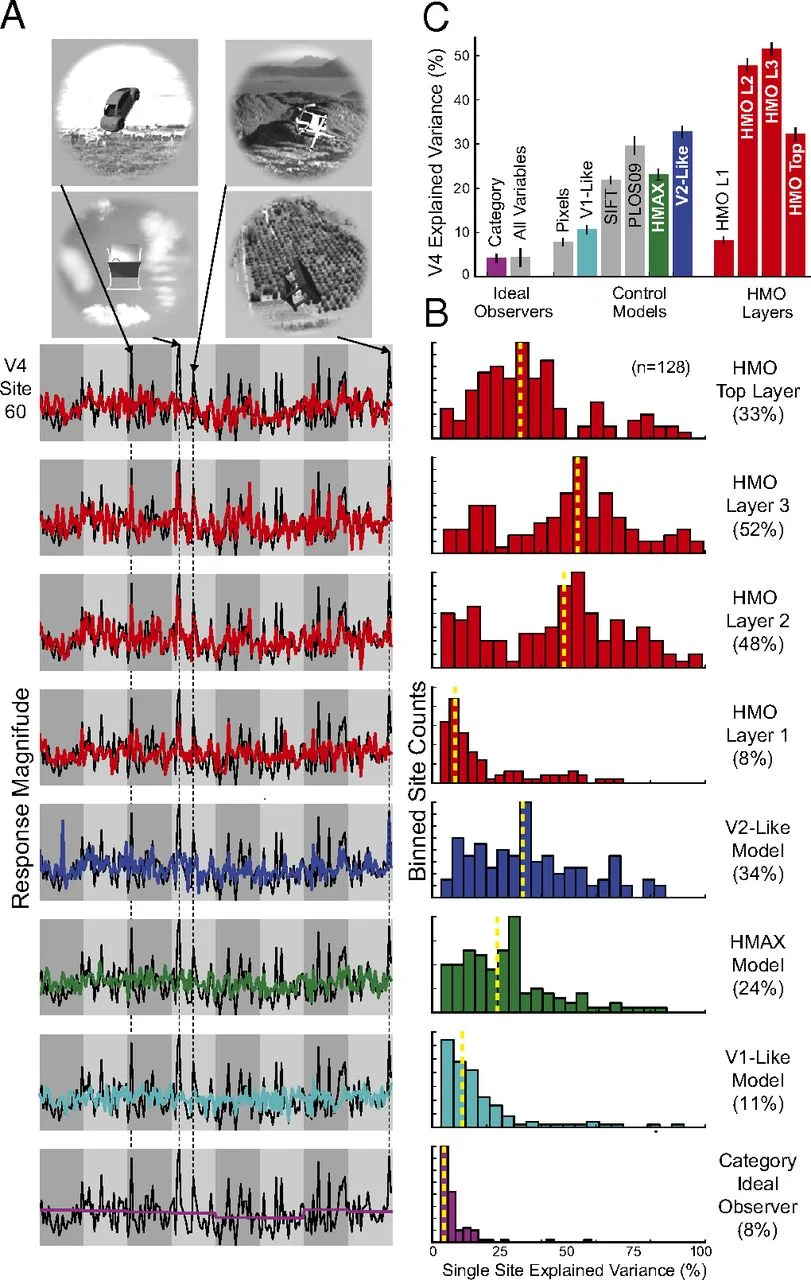
\includegraphics[width=\linewidth]{./img/vision_nn_prediction_v4.png}
                            \caption{Results on V4}
                        \end{subfigure}
                        \caption{
                            \parbox[t]{0.78\linewidth}{
                                (A) Actual neuronal activity (black) and predicted activity (colored).\\
                                (B) $R^2$ value over the population of single IT neurons.\\
                                (C) Median $R^2$ over the population of IT neurons.
                            }
                        }
                    \end{figure}
            \end{itemize}
    \end{descriptionlist}
\end{casestudy}
